%----------
%   WARNING
%----------

% This Guide contains Library recommendations based mainly on APA and IEEE styles, but you must always follow the guidelines of your TFG Tutor and the TFG regulations for your degree.

% THIS TEMPLATE IS BASED ON THE APA STYLE 


%----------
% DOCUMENT SETTINGS
%----------

\documentclass[12pt]{report} % font: 12pt

% margins: 2.5 cm top and bottom; 3 cm left and right
\usepackage[
a4paper,
vmargin=2.5cm,
hmargin=3cm
]{geometry}

% Paragraph Spacing and Line Spacing: Narrow (6 pt / 1.15 spacing) or Moderate (6 pt / 1.5 spacing)
\renewcommand{\baselinestretch}{1.15}
\parskip=6pt

% Color settings for cover and code listings 
\usepackage[table]{xcolor}
\definecolor{azulUC3M}{RGB}{0,0,102}
\definecolor{gray97}{gray}{.97}
\definecolor{gray75}{gray}{.75}
\definecolor{gray45}{gray}{.45}

% PDF/A -- Important for its inclusion in e-Archive. PDF/A is the optimal format for preservation and for the generation of metadata: http://uc3m.libguides.com/ld.php?content_id=31389625. 

% In the template we include the file OUTPUT.XMPDATA. You can download that file and include the metadata that will be incorporated into the PDF file when you compile the memoria.tex file. Then upload it back to your project. 
\usepackage{silence}
\WarningFilter{pdfx}{Setting all color commands to rgb}
\usepackage[a-1b]{pdfx}

% LINKS
\usepackage{hyperref}
\hypersetup{colorlinks=true,
	linkcolor=black, % links to parts of the document (e.g. index) in black
	urlcolor=blue} % links to resources outside the document in blue

% MATH EXPRESSIONS
\usepackage{amsmath,amssymb,amsfonts,amsthm}

% Character encoding
\usepackage{txfonts} 
\usepackage[T1]{fontenc}
\usepackage[utf8]{inputenc}

% English settings
\usepackage[english]{babel} 
\usepackage[babel, english=american]{csquotes}
\AtBeginEnvironment{quote}{\small}

% Footer settings
\usepackage{fancyhdr}
\pagestyle{fancy}
\fancyhf{}
\renewcommand{\headrulewidth}{0pt}
\rfoot{\thepage}
\fancypagestyle{plain}{\pagestyle{fancy}}

% DESIGN OF THE TITLES of the parts of the work (chapters and epigraphs or sub-chapters)
\usepackage{titlesec}
\usepackage{titletoc}
\titleformat{\chapter}[block]
{\large\bfseries\filcenter}
{\thechapter.}
{5pt}
{\MakeUppercase}
{}
\titlespacing{\chapter}{0pt}{0pt}{*3}
\titlecontents{chapter}
[0pt]                                               
{}
{\contentsmargin{0pt}\thecontentslabel.\enspace\uppercase}
{\contentsmargin{0pt}\uppercase}                        
{\titlerule*[.7pc]{.}\contentspage}                 

\titleformat{\section}
{\bfseries}
{\thesection.}
{5pt}
{}
\titlecontents{section}
[5pt]                                               
{}
{\contentsmargin{0pt}\thecontentslabel.\enspace}
{\contentsmargin{0pt}}
{\titlerule*[.7pc]{.}\contentspage}

\titleformat{\subsection}
{\normalsize\bfseries}
{\thesubsection.}
{5pt}
{}
\titlecontents{subsection}
[10pt]                                               
{}
{\contentsmargin{0pt}                          
	\thecontentslabel.\enspace}
{\contentsmargin{0pt}}                        
{\titlerule*[.7pc]{.}\contentspage}  


% Tables and figures settings
\usepackage{multirow} % combine cells 
\usepackage{caption} % customize the title of tables and figures
\usepackage{floatrow} % we use this package and its \ ttabbox and \ ffigbox macros to align the table and figure names according to the defined style.
\usepackage{array} % with this package we can define in the following line a new type of column for tables: custom width and centered content
\newcolumntype{P}[1]{>{\centering\arraybackslash}p{#1}}
\DeclareCaptionFormat{upper}{#1#2\uppercase{#3}\par}
\usepackage{graphicx}
\usepackage{subcaption}
\graphicspath{{figures/}} % images fodler

% Table layout for social sciences and humanities
\captionsetup*[table]{
	justification=centering,
	labelsep=colon,
	labelfont=small,
	singlelinecheck=false,
	labelfont=bf,
	font=small,
	textfont=it
}

% In the preamble
\newcommand{\result}[2]{%
\begin{tabular}{@{}c@{}}
#1\\
(#2)
\end{tabular}
}

% Figure layout for social sciences and humanities
\captionsetup[figure]{
	%name=Figura,
	justification=centering,
	singlelinecheck=true,
	labelsep=newline,
	font=small,
	labelfont=bf,
	textfont=it
}
\floatsetup[figure]{
    style=plaintop,
    heightadjust=caption,
    footposition=bottom,
    font=small
}

% Figures and tables footnote layout 
\captionsetup*[floatfoot]{
    footfont={small, up}
}

% FOOTNOTES
\usepackage{chngcntr} % continuous numbering of footnotes
\counterwithout{footnote}{chapter}

% CODE LISTINGS 
% support and styling for listings. More information in  https://es.wikibooks.org/wiki/Manual_de_LaTeX/Listados_de_código/Listados_con_listings
\usepackage{listings}

% Custom listing
\lstdefinestyle{estilo}{ frame=Ltb,
	framerule=0pt,
	aboveskip=0.5cm,
	framextopmargin=3pt,
	framexbottommargin=3pt,
	framexleftmargin=0.4cm,
	framesep=0pt,
	rulesep=.4pt,
	backgroundcolor=\color{gray97},
	rulesepcolor=\color{black},
	%
	basicstyle=\ttfamily\footnotesize,
	keywordstyle=\bfseries,
	stringstyle=\ttfamily,
	showstringspaces = false,
	commentstyle=\color{gray45},     
	%
	numbers=left,
	numbersep=15pt,
	numberstyle=\tiny,
	numberfirstline = false,
	breaklines=true,
	xleftmargin=\parindent
}

\captionsetup*[lstlisting]{font=small, labelsep=period}
 
\lstset{style=estilo}
\renewcommand{\lstlistingname}{\uppercase{Código}}


% REFERENCES 

% APA bibliography setup
\usepackage[style=apa, backend=biber, natbib=true, hyperref=true, uniquelist=false, sortcites]{biblatex}

\addbibresource{referencias.bib} % The references.bib file in which the bibliography used should be


%-------------
%	DOCUMENT
%-------------

\begin{document}
\hypersetup{pageanchor=false}
\pagenumbering{roman} % Roman numerals are used in the numbering of the pages preceding the body of the work.
	
%----------
%	COVER
%----------	
\begin{titlepage}
	\begin{sffamily}
	\color{azulUC3M}
	\begin{center}
		\begin{figure}[H] % UC3M Logo
			\makebox[\textwidth][c]{
\includegraphics[width=16cm]{logo_UC3M.png}}
		\end{figure}
		\vspace{2.5cm}
		\begin{Large}
			Master Degree in Big Data Analytics\\			
			 2025-2026\\ % Academic year
			\vspace{2cm}		
			\textsl{Master Thesis}
			\bigskip
			
		\end{Large}
		 	{\Huge ``Towards Interpretable Twin Support Vector Machines with Probabilistic Class Membership''}\\
		 	\vspace*{0.5cm}
	 		\rule{10.5cm}{0.1mm}\\
			\vspace*{0.9cm}
			{\LARGE Daniel Del Pozuelo Escalona}\\ 
			\vspace*{1cm}
		\begin{Large}
			Sandra Benítez Peña\\
			Silvia Novo Díaz\\
			Madrid, July 2026\\
		\end{Large}
	\end{center}
	\vfill
	\color{black}
	\fbox{
	\begin{minipage}{0.95\linewidth}
    	\textbf{AVOID PLAGIARISM}\\
    	\footnotesize{The University uses the \textbf{Turnitin Feedback Studio} for the delivery of student work. This program compares the originality of the work delivered by each student with millions of electronic resources and detects those parts of the text that are copied and pasted. Plagiarizing in a TFM is considered a  \textbf{\underline{Serious Misconduct}}, and may result in permanent expulsion from the University.}\end{minipage}}

	% IF OUR WORK IS TO BE PUBLISHED UNDER A CREATIVE COMMONS LICENSE, INCLUDE THESE LINES. IS THE RECOMMENDED OPTION.
	\noindent
\includegraphics[width=4.2cm]{creativecommons.png}\\ % Creative Commons Logo
    \footnotesize{This work is licensed under Creative Commons \textbf{Attribution – Non Commercial – Non Derivatives}}
	
	\end{sffamily}
\end{titlepage}

%----------
%	ABSTRACT AND KEYWORDS 
%----------	
\renewcommand\abstractname{\large\bfseries\filcenter\uppercase{Abstract}}
\begin{abstract}
\thispagestyle{plain}
\setcounter{page}{3}
	The Twin Support Vector Machine (TWSVM) is a powerful state-of-the-art method for supervised binary classification. This thesis investigates the interpretability of TWSVM through the implementation of a probabilistic $L_1$-TWSVM model. By incorporating $L_1$-norm regularization terms into the objective functions, the proposed model promotes sparsity in the weight vectors, thereby enabling independent feature selection for each hyperplane. A bootstrap resampling experiment is conducted to tune the hyperparameters and to evaluate the stability of the proposed model in terms of classification accuracy and probability calibration. The bootstrap experiment also extends the independent feature selection performed by each hyperplane by considering the frequency with which each feature is selected across bootstrap replicates for a given hyperparameter configuration.
	
	
	\textbf{Keywords: Machine Learning, Pattern Classification, Probabilistic Twin Support Vector Machine, Feature Selection, $L_1$-norm}
	
	\vfill
\end{abstract}
	

%----------
%	TOC
%----------	

\tableofcontents
\thispagestyle{fancy}


%----------
%	THESIS
%----------	
\clearpage
\hypersetup{pageanchor=true}
\pagenumbering{arabic} % numbering with Arabic numerals for the rest of the document.	



\chapter{Introduction} \label{chap:intro}

Over the past decade, pattern recognition has become one of the central research areas in machine learning, with applications across domains such as bioinformatics, computer vision, and finance. Pattern recognition is concerned with automatically identifying the underlying structure in data and exploiting such relationships to either predict a specific target variable or uncover hidden structures.

Pattern recognition tasks can be broadly categorized as either \textit{supervised} or \textit{unsupervised}, depending on the availability of a target variable to be predicted. In supervised learning each data instance is associated with a target variable encoding the underlying patterns in data. The objective is to learn a function $f(x)$ that maps input feature vectors, $x$, to their corresponding target, $y$, enabling the prediction of the target values for previously unseen observations. Formally, the training set in supervised learning consists of a collection of pairs, $\{(x_i, y_i)\}_{i=1}^{M}$, where $x_i$ denotes an $N$-dimensional feature vector and $y_i$ represents its associated target. The process of estimating the mapping function $f(x)$ from the training dataset is referred to as learning. Unlike supervised learning, where models are trained using pairs of feature vectors and their corresponding target labels and where such labels are not available during the testing phase, unsupervised learning does not rely on predefined outputs at any stage of the learning process. Unsupervised learning extracts patterns hidden in data without relying on external attributes, such as target variables, explicitly uncovering the underlying structure of the data. The objective of unsupervised learning is not to predict a target variable, but rather to unveil the underlying structure of the data. Typical, unsupervised learning taks include clustering, density estimation and dimensionality reduction, which aim to identify groups of similar instances, estimate the underlying data distribution, or obtain lower-dimensional representations suitable for visualization and analysis.

This thesis is concerned with the interpretability of twin classifiers originally developed for binary classification tasks. As discussed in Section~\ref{chap:supervised-learning}, binary classification arise as a special case of supervised learning in which instances are assigned to one of two possible classes.

In particular, this work investigates the interpretability of the Twin Support Vector Machine (TWSVM) proposed by \cite{khemchandani2007twin} by implementing a probabilistic formulation of the $L_1$-TWSVM. This formulation adapts the probabilistic model introduced by \cite{shao2012probabilistic} for the standard TWSVM and incorporates the $L_1$-TWSVM framework proposed by \cite{bai2014novel}. The inclusion of $L_1$-regularization terms in the objective functions promotes sparsity in the weight vectors, enabling feature selection.

\newpage

The current context of increasing data availability motivates the application of feature selection strategies to efficiently deploy machine learning models. Feature selection identifies the most relevant variables contributing to the classification task, addressing a key challenge in data-driven decision making. Moreover, feature selection provides a dual advantage, as it removes irrelevant or redundant features, leading to a reduction in data dimensionality. This, in turn, improves computational efficiency and can enhance classification performance by removing irrelevant or noisy features.

As the TWSVM is based on the well-known Support Vector Machine (SVM) paradigm, it naturally produces hard-label classifications. That is, SVM-based models assign each instance to a specific class based on distance comparisons to the decision boundary. The motivation behind introducing a probabilistic formulation of the TWSVM is to provide a measure of confidence in the model's predictions, improving interpretability and reliability.

This work proposes a bootstrap experiment to explore an extensive grid of hyperparameter values for tuning the model, while enforcing a stability analysis of the probability calibration produced by the model. Following the $L_1$-TWSVM formulation proposed by \cite{bai2014novel}, this study investigates an independent feature selection strategy for each hyperplane, providing additional interpretability of the model behavior. This strategy is further exploited through heatmap representations, which illustrate the selection frequency of each feature for each hyperplane across the different bootstrap replicates generated in the proposed experiment. This work further presents an empirical comparison between the standard linear SVM, the standard TWSVM, and the proposed probabilistic $L_1$-TWSVM using several benchmark datasets from the University of California, Irvine (UCI) Machine Learning Repository.

This thesis is organized as follows. A brief review of supervised learning techniques is presented in Section~\ref{chap:supervised-learning}, whereas feature selection strategies are revisited in Section~\ref{chap:feature-selection}. Section~\ref{chap:foundations-twsvm} presents the foundations of the Twin Support Vector Machine (TWSVM), discussing its relationship with the well-known SVM framework as well as its immediate connection to the GEPSVM model. The bootstrap experiment and the proposed feature selection strategy are described in Section~\ref{chap:methodology}, while the experimental setup is presented in Section~\ref{chap:experiment}. Finally, Section~\ref{chap:results} presents the results, and Section~\ref{chap:conclusions} provides the conclusions of the thesis.



\chapter{Supervised learning techniques} \label{chap:supervised-learning}

As introduced in Section \ref{chap:intro}, supervised learning defines a class of problems in which the training data consists of pairs of input feature vectors and their corresponding target vectors. The objective is to learn a function that generalizes the mapping between inputs and targets observed during training, enabling the prediction of previously unseen target values instances during evaluation. Supervised learning problems can generally be categorized as either \textit{regression} or \textit{classification} tasks, depending on the nature of the target variable. Regression problems arise when the target consists of one or more continuous real-valued variables. In contrast, in supervised classification problems, the target to be predicted is a discrete variable belonging to a finite set of N categories.


\section{Regression} \label{sec:regression}

As stated above, regression constitutes a supervised learning paradigm in which the dataset consists of pairs of input feature vectors and their corresponding target variables, where the target is typically a continuous real-valued quantity, $y \in R$ or in the multivariate case, a vector-valued output $y \in R^n$. Another typical setting for regression is time series analysis, in which the objective is to predict future values of a temporally ordered variable based on its own past observations or the past values of related exogenous variables. Although the literature on regression methods is extensive and includes a wide variety of approaches ranging from linear parametric models such as Ordinary Least Squares, Ridge Regression, Lasso Regression, and Elastic Net, to instance-based methods such as k-Nearest Neighbors, the focus on interpretability in this thesis primarily motivates the distinction between tree-based methods and score-based methods.


Tree-based algorithms recursively partition the input feature space into increasingly homogeneous regions. In the context of regression, decision tree methods can generally be categorized into two main groups: regression trees and model trees. In regression trees, each terminal node, termed as leaf, stores a specific continuous-valued prediction, typically corresponding to the mean value of the target variable for the training instances reaching that leaf. In contrast, model trees associate linear regression models with their terminal nodes, allowing the final prediction to be obtained from locally fitted models. Consequently, model trees are capable of representing more complex non-linear relationships while preserving a certain degree of interpretability. Regression trees determine the optimal split by minimizing the variability of the target variable within the resulting partitions. Common splitting criteria include variance reduction and standard deviation reduction (\cite{hastie2009elements}).

\newpage

Motivated by regularized regression approaches such as Ridge Regression, where a penalty term is introduced to control model complexity, score-based methods including the Support Vector Regression (SVR), introduced by \cite{cortes1995support}, cast the supervised regression problem as the minimization of a regularized objective function. In this context, standard SVR employs the $\epsilon$-insensitive loss function, which does not penalize deviations between the prediction and the target as long as their absolute difference remains below a predefined threshold $\epsilon$ (\cite{bishop2006pattern}).

The performance of regression models is typically assessed using evaluation metrics such as the Mean Absolute Error (MAE), which measures the average magnitude of prediction errors and is generally less sensitive to the presence of outliers. In contrast, the Mean Squared Error (MSE) and its square root counterpart, the Root Mean Squared Error (RMSE), are more sensitive to outliers, as they assign a higher penalty to larger deviations. Both MAE and RMSE are scale-dependent metrics, meaning that their values are expressed in the same units as the target variable. By contrast, the MSE expresses the error in squared units of the target variable.


\section{Classification} \label{sec:classification}

Supervised classification problems arise in applications where the dataset consists of pairs of input feature vectors and target variables, the latter being discrete variables that take values from a finite set of N categories. Binary classification arises as a particular case of supervised classification in which the target variable comprises exactly two classes. Analogously to the regression case, and motivated by the interpretability focus of this thesis, the discussion is primarily centered on the distinction between tree-based and score-based methods.

Tree-based algorithms for classification proceed similarly to those for regression as they recursively partition the dataset, aiming to produce increasingly homogeneous subsets. However, unlike decision trees for regression, which select the splitting attribute at each node by minimizing measures of dispersion such as variance or standard deviation within the resulting partitions, decision trees for classification select the optimal splitting attribute by maximizing class purity. This is typically achieved by minimizing impurity measures such as entropy or the Gini index, or equivalently by maximizing information gain.

Traditionally, score-based methods for classification, such as the Support Vector Machine (SVM) and the Twin Support Vector Machine (TWSVM), in which this thesis is focused, were originally developed for the binary classification setting and were later extended to the general multiclass case involving a discrete target variable with N distinct categories. 

\newpage

In general, score-based methods formulate the classification problem by learning a decision function that partitions the input feature space into regions corresponding to the target classes through the optimization of a scoring function. In the case of the standard linear SVM, this scoring function is defined in terms of the geometric margin, i.e., the Euclidean distance from the decision boundary (the separating hyperplane) to the closest training instances of each class. Similarly, the standard TWSVM formulation involves solving two optimization problems, in which the scoring functions are defined by fitting proximal hyperplanes to the data points of each class.

The performance of classification methods can be evaluated using metrics such as classification accuracy, F1-score, precision, and recall when the model produces hard-label outputs, as its natural in SVM-based methods, i.e., when each instance is strictly assigned to a single class. In the binary classification setting, precision and recall are particularly relevant, as they allow the evaluation of model performance under cost-sensitive scenarios, where the cost of misclassifying an instance of one class is higher than the cost of misclassifying it as the opposite class. These metrics are defined as:

\begin{subequations}
\begin{minipage}[c]{0.40\textwidth}
\begin{equation}
acc = \frac{1}{M} \sum_{i=1}^{M} 1[\hat{y}_i = y_i]
\end{equation}
\end{minipage}
\begin{minipage}[c]{0.40\textwidth}
\begin{equation}
F1 = \frac{\text{2TP}}{\text{2TP} + \text{FP} + \text{FN}}
\end{equation}
\end{minipage}
\label{eq:calibration_metrics}
\end{subequations}

where TP denotes the number of true positives, i.e., the number of instances correctly classified as belonging to the positive class. FP denotes the number of false positives,namely the instances incorrectly classified as positive, while FN denotes the number of false negatives, i.e., instances incorrectly classified as negative.

As discussed in Section \ref{chap:intro}, the introduction of probabilistic formulations for score-based methods such as the linear SVM and the TWSVM is motivated by the need to assess and calibrate model confidence, improving interpretability and reliability. In particular, the calibration of probabilistic classifiers is traditionally evaluated using proper scoring rules such as the Brier Score (BS) or negative log-likelihood (NLL). Consider a binary classification setting with $M$ observations, where the labels are defined as $y_i \in \{0,1\}$. The calibration metrics introduced above can then be expressed as follows:

\begin{subequations}
\begin{minipage}{0.40\textwidth}
\begin{equation}
BS = \frac{1}{M} \sum_{i=1}^{M} (y_i - \hat{p}_{i,+1})^2
\end{equation}
\end{minipage}
\begin{minipage}{0.40\textwidth}
\begin{equation}
NLL = - \frac{1}{M} \sum_{i=1}^{M} \log \left( \hat{p}_{i,y_i} \right)
\end{equation}
\end{minipage}
\label{eq:calibration_metrics}
\end{subequations}

where $\hat{p_{i,+1}}$ denotes the predicted probability that the i-th instance belongs to the positive class, and $\hat{p_{i,y_i}}$ denotes the predicted probability assigned to the true class label, $y_i$. 

For brevity's sake, this thesis focuses exclusively on the binary supervised classification setting, in which the input space is partitioned into two disjoint classes. Accordingly, the label set is restricted to $C = \{-1, +1\}$, representing the so-called negative and positive classes, respectively.



\chapter{Feature Selection methods} \label{chap:feature-selection}

Nowadays, feature selection has become an essential component of modern classification methods, particularly when the number of available attributes, N, is large. Neither the linear SVM nor the standard TWSVM performs feature selection automatically, as both methods are typically based on quadratic regularization. Feature selection restricts the degrees of freedom available to the classifier, thereby controlling model complexity and reducing the risk of overfitting. Furthermore, by limiting the number of attributes included in the model, feature selection can significantly reduce computational costs and improve the efficiency of the learning process. As mentioned above, the removal of noisy or redundant features may also enhance the classification accuracy of the models (\cite{hastie2009elements}). This section briefly reviews the different feature selection methods, emphasizing the distinctions among filter, wrapper, and embedded approaches, motivating the adoption of an embedded feature selection method in this thesis.


\section{Filter methods} \label{sec:filter-methods}

Given a set of features, filter methods evaluate the importance of each attribute individually by measuring its dependence on the target variable. The features are subsequently ranked according to a predefined scoring criterion, and the least informative ones are discarded. A wide variety of methods has been proposed in the literature for computing relevance indices, such as the Fisher score, mutual information, information gain, and the Laplacian score. Filter methods do not incorporate learning; i.e., they are independent of the predictor model itself. Generally, these methods are applied during the preprocessing stage, while the number of selected features is treated as a hyperparameter to be tuned (\cite{zaki2014data}).


\section{Wrapper methods} \label{sec:wrapper-methods}

Wrapper methods assess the relevance of features by evaluating subsets of attributes rather than considering each feature individually. To identify an appropriate subset, these methods employ search strategies such as sequential forward selection or sequential backward elimination, avoiding the exhaustive evaluation of all possible feature combinations, which becomes computationally infeasible in most applications. The quality of each candidate subset is assessed by training and validating a machine learning algorithm, typically using a cross-validation scheme. The learning algorithm used in wrapper methods serves solely as a performance estimator for assessing the quality of candidate feature subsets, without exploiting any knowledge of its internal structure (\cite{guyon2006feature}).


\section{Embedded methods} \label{sec:embedded-methods}

While filter methods do not interact with the learning process and wrapper methods decouple the evaluation of feature subsets from the training of the final predictive model, embedded methods perform feature selection as an integral part of the model training procedure. In this sense, embedded approaches exploit knowledge of the internal structure of the learning algorithm to perform feature selection directly during the optimization process. Depending on the predictive model considered, specific embedded feature selection techniques are designed to identify a feature subset of a given size that yields optimal generalization performance. One of the most common embedded strategies consists of implementing a greedy algorithm that iteratively adds or removes features from the candidate subset, approximating the optimal feature subset that minimizes the expected risk, maximizing the model's generalization ability (\cite{zaki2014data}).

Section \ref{sec:fs-twsvm} discusses embedded feature selection methods specifically integrated into the standard TWSVM model. The feature selection approach implemented in this thesis, originally proposed by \cite{bai2014novel}, can be regarded as one of the simplest embedded feature selection strategies for TWSVM. It induces sparsity in the weight vectors of the TWSVM by incorporating $L_1$-regularization terms into the objective functions, resulting in an $L_1$-TWSVM formulation. This formulation promotes the selection of relevant features for each hyperplane by shrinking the weights of irrelevant features to zero. In this way, the method exploits the internal structure of the model to perform feature selection during training, thereby identifying relevant feature subsets associated with each separating hyperplane. The remaining embedded feature selection approaches discussed in Section \ref{sec:fs-twsvm} are referred to as \textit{joint} feature selection methods, since they select a single optimal feature subset simultaneously for both hyperplanes. The work by \cite{maldonado2017synchronized} is particularly noteworthy for exploring such approaches in the context of twin classifiers.



\chapter{Theoretical foundations of Twin Support Vector Machines} \label{chap:foundations-twsvm}

The Twin Support Vector Machine (TWSVM) proposed by \cite{khemchandani2007twin} is based on the key idea of determining two non-parallel proximal hyperplanes, each adjusted to fit the observations of one class while maintaining maximal separation from the observations of the opposite class. This idea stems from the Generalized Eigenvalue Proximal Support Vector Machine (GEPSVM) formulation developed by \cite{mangasarian2006multisurface}. However, unlike GEPSVM, the model proposed by \cite{khemchandani2007twin} departs from generalized eigenvalue problems, instead following a formulation based on quadratic programming, similar to that used in standard linear SVMs. The similarities in the quadratic programming problems defining the hyperplanes in TWSVM motivate the discussion of SVM and GEPSVM methods in the first part of this section. Subsequently, the standard TWSVM formulation, feature selection methods for TWSVM, and a probabilistic model for TWSVM are presented.
 

\section{Support Vector Machine theory} \label{sec:svm-theory}

The Support Vector Machine (SVM), introduced by \cite{vapnik1998statistical}, remains one of the most influential methods in supervised pattern classification. Rooted in statistical learning theory, the SVM paradigm has become one of the state-of-the-art frameworks in modern machine learning due to its solid theoretical foundations and versatility across a wide range of classification and regression tasks (\cite{khan2012novel,lin2006method}).

In its simplest version, the linear SVM defines a linear discriminant function, $f(x) = w^{T}x+b$ as a classifier. Among the infinitely many separating hyperplanes, the linear SVM selects the one that maximizes the geometric margin defined as the minimum distance between the hyperplane and the closest training instances, known as the support vectors. The parameters $w$ and $b$ are obtained by solving a convex quadratic programming problem (QPP) subject to linear inequality constraints. The soft margin primal formulation of the linear SVM (\cite{bishop2006pattern, cristianini2000introduction}) is given by

\begin{equation}
\begin{aligned}
\min_{w,b} \quad \frac{1}{2}\|w\|^{2} + C\sum_{i=1}^{M}\xi_i
\quad \text{s.t} \quad & y_i(w^{T}x_i+b) \geq 1-\xi_i \\
& \xi_i \geq 0\quad \forall i = \{1,\dots,M\}
\label{eq:svm_primal}
\end{aligned}
\end{equation}

where the regularization parameter $C >0$ controls the trade-off between margin maximization and the penalization of margin violations through the non-negative slack variables $\xi_i$. 

\newpage

Despite its higher computational complexity, scaling with the size of the training dataset (\cite{chapelle2007training}), the use of the dual formulation remains the predominant approach as it enables the incorporation of kernel functions. The dual formulation is given by (\cite{hofmann2006support})

\begin{equation}
\begin{aligned}
\max_{\alpha} \quad & -\frac{1}{2}\sum_{i=1}^{M}\sum_{j=1}^{M}\alpha_i\alpha_jy_iy_jx_i^{T}x_j + \sum_{i=1}^{M}\alpha_i \\
\text{s.t.} \quad & \sum_{i=1}^{M}\alpha_iy_i = 0 \\
\quad  & 0 \leq \alpha_i \leq C \quad \forall i \in \{1,\dots, M\}
\label{eq:svm_dual}
\end{aligned}
\end{equation}

where $\alpha_i$ denotes the dual coefficient associated with the i-th training sample. The dual formulation facilitates the introduction of kernels through the replacement of inner products between input vectors with kernel evaluations $K(x_i, x_j)$. This so-called kernel trick enables the implicit mapping of the data into a higher-dimensional feature space, in which classes that are not linearly separable in the original input space may become linearly separable.

With the increasing availability of large-scale datasets, several extensions of the SVM paradigm have been proposed to improve computational efficiency. Regarding binary data classification, the Generalized Eigenvalue Proximal Support Vector Machine (GEPSVM), introduced by \cite{mangasarian2006multisurface}, significantly reduced computational complexity by reformulating the classification problem as a generalized eigenvalue problem. Moreover, GEPSVM has been shown to outperform standard SVM methods in certain nonlinearly separable classification tasks, such as the Exclusive OR (XOR) problem.

At the time GEPSVM was introduced, it was motivated by the Proximal Support Vector Machine (PSVM) proposed by \cite{fung2001proximal}. In contrast to the standard SVM, which determines a single maximum-margin separating hyperplane, PSVM constructs two parallel class-specific proximal hyperplanes, each being fitted to one class while remaining as far as possible from the other. GEPSVM generalizes this approach by removing the parallelism constraint, allowing the resulting proximal hyperplanes to be non-parallel.

Consider the previous binary classification setting. Let $A \in R^{m_1xN}$ denote the matrix containing all observations belonging to the positive class, $y_i = +1$, and let $B \in R^{m_2xN}$ denote the matrix containing all the observations belonging to the negative class, $y_i = -1$. Here, $m_1$ and $m_2$ denote the number of observations in the positive and negative classes, respectively, with $m_1 + m_2 = M$.

\newpage

GEPSVM seeks two non-parallel proximal hyperplanes, $x^{T}w_1-\gamma_1 = 0$ and $x^{T}w_2 -\gamma_2 = 0$, where $w_k \in R^{N}$ and $\gamma_k \in R$ for $k = 1,2$. Each hyperplane is constructed to be proximal to the observations of one class while remaining as distant as possible from the observations of the opposite class.

Originally, GEPSVM estimates the coefficients $w_k$ and $\gamma_k$ for $k = 1,2$, by minimizing, for each class, the normalized sum of squared Euclidean distances from the observations of that class to the corresponding hyperplane while maximizing the normalized sum of squared Euclidean distances from the observations of the opposite class. The normalization terms in the original GEPSVM formulation cancel out, yielding the following objective functions expressed as ratios of within-class and between-class squared residuals. Furthermore, the GEPSVM formulation includes Tikhonov regularization terms, namely $\delta(\|w_1\|_2^{2}+\gamma_1^{2})$ and $\delta(\|w_2\|_2^{2}+\gamma_2^{2})$, to mitigate singularity issues in the resulting generalized eigenvalue problems. The resulting optimization problems can be expressed as

\begin{subequations}
\begin{align}
& \min_{(w_1,\gamma_1)} \quad \frac{\|Aw_1-e\gamma_1\|_2^{2} + \delta(\|w_1\|_2^{2}+\gamma_1^{2})}{\|Bw_1 -e\gamma_1\|_2^{2}} \\
& \min_{(w_2,\gamma_2)} \quad \frac{\|Bw_2-e\gamma_2\|_2^{2} + \delta(\|w_2\|_2^{2}+\gamma_2^{2})}{\|Aw_2 -e\gamma_2\|_2^{2}}
\label{eq:gepsvm}
\end{align}
\end{subequations}

Geometrically, each hyperplane is obtained by minimizing its total squared distance to one class while maximizing its relative distance to the opposite (\cite{mangasarian2006multisurface}). The optimization problem associated with the first hyperplane can be reformulated in terms of the symmetric matrices, $G = \begin{bmatrix} A\;\;e \end{bmatrix}^{T} x \begin{bmatrix} A\;\;e\end{bmatrix} + \delta I$ and $H = \begin{bmatrix} B\;\;e \end{bmatrix}^{T} x \begin{bmatrix} B\;\;e \end{bmatrix}$, where $G, H \in R^{(N+1)x(N+1)}$. The optimization problem associated with the second hyperplane can be derived by introducing two symmetric matrices $L, M \in R^{(N+1)x(N+1)}$, defined analogously to $G$ and $H$, with the roles of the matrices A and B reversed. Consequently, both optimization problems can be expressed as Rayleigh quotients of the form

\begin{subequations}
\begin{minipage}{0.38\textwidth}
\begin{equation}
\min_{z_1 \neq 0} \frac{z_1^{T}Gz_1}{z_1^{T}Hz_1}
\end{equation}
\end{minipage}
\hspace{0.1cm}
\begin{minipage}{0.36\textwidth}
\begin{equation}
\min_{z_2 \neq 0} \frac{z_2^{T}Lz_2}{z_2^{T}Mz_2}
\end{equation}
\end{minipage}
\label{eq:gepsvm_rayleigh}
\end{subequations}

where, $z_1 = \begin{bmatrix}
w_1\\ \gamma_1\end{bmatrix}$ and $z_2 = \begin{bmatrix}
w_2\\ \gamma_2\end{bmatrix}$.

By the minimization property of generalized Rayleigh quotients (\cite{parlett1998symmetric}) the global minimum of each optimization problem in Equation \ref{eq:gepsvm_rayleigh} is given by the eigenvector associated with the smallest generalized eigenvalue of the corresponding generalized eigenvalue problem:

\begin{subequations}
\begin{minipage}{0.38\textwidth}
\begin{equation}
Gz_1 = \lambda_1 Hz_1
\end{equation}
\end{minipage}
\begin{minipage}{0.38\textwidth}
\begin{equation}
Lz_2 = \lambda_2 Mz_2
\end{equation}
\end{minipage}
\end{subequations}

The resulting eigenvectors, $z_1$ and $z_2$, determine the non-parallel proximal hyperplanes, $x^{T}w_1+\gamma_1 = 0$ and $x^{T}w_2 + \gamma_2 = 0$. Recent advances in GEPSVM have focused on improving its robustness by reformulating the generalized eigenvalue problems as standard eigenvalue problems, as proposed by \cite{ye2009improved}.


\section{Twin Support Vector Machines} \label{sec:twsvm}

As stated above, the GEPSVM method developed by \cite{mangasarian2006multisurface} inspired several improvements. Motivated by GEPSVM, \cite{khemchandani2007twin} proposed a novel binary classification method termed the Twin Support Vector Machine (TWSVM), which retains the fundamental idea of learning a pair of non-parallel proximal hyperplanes, each associated with the instances of one of the classes. Although TWSVM pursues the same underlying objective as GEPSVM, its formulation replaces the generalized eigenvalue problems with a pair of quadratic programming problems (QPPs). The formulation of each QPP is closely related to that of the standard linear SVM, except that not all the training instances appear simultaneously in both the objective function and the constraints. Precisely, for the hyperplane associated with a given class, only the instances of that class contribute to the objective, whereas the instances of the opposite class appear exclusively on the linear constraints. As a result, the two optimization problems solved by TWSVM are computationally smaller than the single QPP required in the standard SVM formulation. \cite{khemchandani2007twin} reported that TWSVM is up to four times faster than the standard SVM on certain benchmark datasets. Furthermore, as in the case of GEPSVM, TWSVM has demostrated improved performance on XOR-type problems.

Recall the binary supervised classification setting introduced in the discussion of the GEPSVM at Section \ref{sec:svm-theory}. In this context, the TWSVM algorithm seeks to construct two non-parallel hyperplanes in the given N-dimensional input space, namely $x^Tw_1+b_1 = 0$ and $x^Tw_2+b_2 = 0$. Each of these hyperplanes is designed to be as close as possible to the samples of its corresponding class while remaining as far as possible from the samples of the opposite class.

Requiring each hyperplane to be as close as possible to the samples of its own class is equivalent to minimizing the sum of squared distances from the instances of a given class to their corresponding hyperplane. This leads to the following QPPs:

\begin{subequations}
\begin{align}
\min_{w_1,b_1} \sum_{i \in A} (x_i^T w_1 + b_1)^2 
&= \min_{w_1,b_1} \frac{1}{2}\|Aw_1 + e_1 b_1\|_2^2 \\
\min_{w_2,b_2} \sum_{j \in B} (x_j^T w_2 + b_2)^2 
&= \min_{w_2,b_2} \frac{1}{2}\|Bw_2 + e_2 b_2\|_2^2
\label{eq:twsvm_ls}
\end{align}
\end{subequations}

where, $e_i \in R^{m_i}$ denotes a vector of ones of appropiate dimension. These QPPs correspond to least-squares formulations of the linear systems $Aw_1+e_1b_1 = 0$ and $Bw_2+e_2b_2 = 0$.

\newpage

Since the zero vector is a feasible solution of the corresponding homogeneous least-squares problems, the previous unconstrained QPPs admit the trivial solution. Thus, without additional constraints, both optimization problems collapse to a degenerate solution corresponding to a trivial hyperplane. This degeneracy is prevented by introducing the following constraints in both QPPs. Furthermore, these constraints enforce a unit functional margin with respect to the samples of the opposite class.

\begin{subequations}
\begin{align}
\min_{w_1,b_1} \frac{1}{2}\|Aw_1+e_1b_1\|_2^2
& \quad \text{s.t. } -(Bw_1+e_2b_1) \geq e_2 \\
\min_{w_2,b_2} \frac{1}{2}\|Bw_2+e_2b_2\|_2^2
& \quad \text{s.t.  }\; Aw_2+e_1b_2 \geq e_1
\end{align}
\label{eq:twsvm_ls_constraints}
\end{subequations}

For example, the constraint associated with the positive-class hyperplane, $-(Bw_1+e_2b_1) \geq e_2$, imposes that $-(x_j^Tw_1 + b_1) \geq 1\,\,\forall x_j\in B$ and hence $x_j^Tw_1+b_1 \leq -1$. As a result, all instances belonging to the negative class are required to lie on the negative side of the positive-class hyperplane while satisfying the unit functional-margin constraint.

The formulation presented in Equation \ref{eq:twsvm_ls_constraints} corresponds to the hard-margin version of the standard TWSVM method proposed by \cite{khemchandani2007twin}, as it implicitly assumes that the classes are strictly separable. Specifically, it assumes the existence of two non-parallel proximal hyperplanes satisfying the corresponding unit functional-margin constraints, namely $-(Bw_1+e_2b_1)\geq e_2$ and $Aw_2+e_1b_2 \geq e_1$. However, strict separability rarely holds in practice. Thus, it is standard practice to relax the hard-margin formulation in order to accommodate a certain degree of overlap between classes, thereby permitting some observations to violate the separation constraints.

Allowing violations of the separation constraints entails accepting a certain degree of margin violation and, potentially, misclassification. As in the standard soft-margin SVM formulation, such violations are accommodated through the introduction of non-negative slack variables, $\xi_1 \in R^{m_1}$ and $\xi_2 \in R^{m_2}$, satisfying $\xi_1\geq 0$ and $\xi_2 \geq 0$. The introduction of these slack variables modifies the separation constraints as follows:

\begin{subequations}
\begin{align}
-&(Bw_1+e_2b_1) \geq e_2 - \xi_2 \\
& (Aw_2+e_1b_2) \geq e_1 - \xi_1
\end{align}
\end{subequations}

where $\xi_2$ permits violations of the separation constraints for the negative samples to the positive-class hyperplane, while $\xi_1$ imposes analogous relaxed constraints for the positive samples with respect to the negative-class hyperplane.

\newpage

Unlike standard SVM, which determines class membership using a single separating hyperplane, TWSVM classifies samples based on their relative distances to the two class-specific hyperplanes. As a result, the separation constraints, and hence the role of the slack variables in TWSVM, are interpreted in terms of the functional margin rather than the geometric margin used in standard SVM.

For example, consider the i-th slack variable associated with the positive-class hyperplane, denoted by $\xi_{2,i}$. A zero slack variable, $\xi_{2,i} = 0$, indicates that the i-th observation satisfies the unit functional-margin constraint with respect to the positive-class hyperplane. A positive slack variable satisfying $0<\xi_{2,i}< 1$ indicates that the observation lies within the functional-margin region while remaining on the correct side of the positive-class hyperplane. When $\xi_{2,i} = 1$ and the corresponding constraint is active, the observation lies on the decision boundary, $x_i^{T}w_1 + b_1 = 0$. Finally, $\xi_{2,i} > 1$ indicates that the observation has crossed the decision boundary and is therefore misclassified.

Analogous to the standard soft-margin SVM formulation, in the soft-margin TWSVM the slack variables are incorporated into the objective functions for each proximal hyperplane through linear penalty terms, $e_2^{T}\xi_2$ and $e_1^{T}\xi_1$, respectively. The hyperparameters $c_1$ and $c_2$ define the trade-off between minimizing the least-squares fitting error for the corresponding class and penalizing violations of the separation constraints.

Finally, the standard TWSVM algorithm solves the following pair of QPPs (\cite{khemchandani2007twin}):

\begin{subequations}
\label{eq:soft_margin_twsvm}
\begin{align}
&\min_{w_1, b_1, \xi_2} \quad \frac{1}{2}\|A w_1 + e_1 b_1\|^2 + c_1 e_2^T \xi_2 \\
\quad & \text{s.t. } \quad -(B w_1 + e_2 b_1) + \xi_2 \geq e_2, \nonumber\\
& \quad \quad \quad \quad \xi_2 \geq 0 \nonumber
\nonumber \\[2ex]
& \min_{w_2, b_2, \xi_1} \quad \frac{1}{2}\|B w_2 + e_2 b_2\|^2 + c_2 e_1^T \xi_1 \\
& \quad \text{s.t. }  \quad A w_2 + e_1 b_2 + \xi_1 \geq e_1, \nonumber \\
&\quad \quad \quad \quad \xi_1 \geq 0 \nonumber
\end{align}
\end{subequations}

As shown above, the TWSVM formulation replaces the margin-maximization principle of standard linear SVMs with a proximal least-squares fitting approach, whereby instances from each class are expected to cluster around their corresponding proximal hyperplane.

\newpage

\section{Feature Selection in Twin Support Vector Machines} \label{sec:fs-twsvm}

The competitive performance exhibited by TWSVMs, together with their lower computational cost compared with standard SVM methods, makes them particularly suitable in the current context of increasingly large datasets. However, their effectiveness may be compromised in high-dimensional settings due to the presence of irrelevant features. Within the standard SVM framework, several feature selection methods have been proposed to discard irrelevant variables, thereby improving computational efficiency through a reduction in the dimensionality of the input space.

Feature selection methods developed for standard SVMs rely on the single weight assigned to each feature by the maximum-margin separating hyperplane (\cite{chang2008feature}). TWSVM, however, generates two class-specific hyperplanes, providing two distinct weights to each feature. This dual representation prevents the direct application of standard SVM feature selection methods to TWSVM.

Motivated by the success of $L_1$-SVMs in feature selection, \cite{bai2014novel} proposed an $L_1$-TWSVM formulation that incorporates $L_1$-norm regularization into the optimization problems defining the two class-specific proximal hyperplanes. The induced sparsity in the weight vectors enables feature selection to be performed independently for each hyperplane. Consequently, coefficients corresponding to irrelevant or redundant features are shrunk to zero, thereby reducing the dimensionality of the model and enhancing its interpretability.

Following their proposed $L_1$-TWSVM formulation, \cite{bai2014novel} introduce a diagonal matrix that enables the joint penalization of the weights associated with each feature across both hyperplanes. As a result, the two optimization problems defining the hyperplanes were reformulated as a single multi-objective mixed-integer programming problem (MOMIPP), yielding a joint feature selection strategy for both hyperplanes. Similarly, \cite{maldonado2017synchronized} proposed a joint feature selection method for the Nonparallel Hyperplane SVM (NH-SVM), a twin classifier that generates both non-parallel proximal hyperplanes by solving a single optimization problem. By exploiting this compact formulation, the authors incorporated $L_\infty$-norm regularization terms that jointly penalize the coefficients associated with each feature across the two hyperplanes, thereby enforcing simultaneous feature selection for both decision functions.

\newpage

Despite the joint feature selection methods for twin classifiers discussed above, the focus of the present work on the interpretability of TWSVMs motivates the use of the $L_1$-TWSVM formulation originally proposed by \cite{bai2014novel} presented in Equation \ref{eq:basic_l1_twsvm}. $L_1$-TWSVM enables independent feature selection for each proximal hyperplane, hence identifying distinct sets of features that characterize the two class-specific hyperplanes.

\begin{subequations}
\label{eq:basic_l1_twsvm}
\begin{align}
& \min_{w_1, b_1, \xi_2} \quad \|w_1\|_1 + c_1\|Aw_1+e_1b_1\|_1 + c_3e_2^T\xi_2 \\
& \quad \text{s.t } \quad -(Bw_1+e_2b_1) \geq e_2 - \xi_2,\nonumber \\
& \quad \quad \quad \quad \xi_2 \geq 0 \nonumber\\
\nonumber \\[2ex]
& \min_{w_2, b_2, \xi_1} \quad \|w_2\|_1 + c_2\|Bw_2+e_2b_2\|_1 + c_4e_1^T\xi_1 \\
& \quad \text{s.t } \quad (Aw_2+e_1b_2) \geq e_1 - \xi_1, \nonumber\\
& \quad \quad \quad \quad \xi_1 \geq 0 \nonumber
\end{align}
\end{subequations}

As discussed above, the $L_1$-TWSVM formulation introduces an $L_1$-norm regularization term for the weight vector of each hyperplane, promoting sparsity in the resulting solutions. Furthermore, the least-square fitting term associated with each hyperplane is replaced by an $L_1$-norm fitting term. Unlike the standard TWSVM formulation, where the contribution of the fitting term in each objective function is fixed at $\frac{1}{2}$ and the penalty associated with margin violations is controlled by a single hyperparameter, the proposed $L_1$-TWSVM introduces two hyperparameters for each objective function. These hyperparameters independently control the influence of the fitting term and penalty term, providing greater flexibility.

The previously presented $L_1$-TWSVM formulation defines two nondifferentiable programming problems due to the presence of nonlinear terms in the objective functions. Specifically, for the first hyperplane terms such as $\|w_1\|_1 = \sum_{n=1}^N|w_n^{(1)}|$ and $\|Aw_1+e_1b_1\|_1 = \sum_{i=1}^{m_1}|\sum_{n=1}^Na_{i,n}w_n^{(1)} + b_1|$ introduce nondifferentiability into the objective function. Analogous nondifferentiable terms arise in the optimization problem associated with the second hyperplane.

Following, \cite{bai2014novel}, these problems can be transformed into differentiable linear programming problems (DLPPs), which can be solved using the well-known simplex algorithm, by introducing the following auxiliary variables, $w_i = p_i - q_i$ for $i = 1,2$ as well as, $Aw_1 + e_1b_1 = s_1 - t_1$ and $Bw_2 + e_2b_2 = s_2 - t_2$.

\newpage

The auxiliary variables introduce a positive-negative decomposition of the weight vectors and fitting terms, whereby each variable is expressed as the difference of two nonnegative variables. The following reformulation allows absolute values to be represented as the sum of these components, yielding a linear formulation of the $L_1$-TWSVM (\cite{bai2014novel}).

\begin{subequations}
\begin{align}
& \min_{p_1,q_1,s_1,t_1,b_1,\xi_2} \quad e_1^T(p_1 + q_1) + c_1e_1^T(s_1 + t_1) + c_3e_1^T\xi_2 \\
& \quad \quad \quad \;\;\begin{aligned}
\text{s.t.} \quad 
& A(p_1 - q_1) + e_1b_1 = s_1 - t_1, \\
& -B(p_1 - q_1) + e_2b_1 \geq e_2 - \xi_2, \\
& p_1, q_1, s_1, t_1, \xi_2 \geq 0
\nonumber \end{aligned}
\\[2ex]
& \min_{p_2,q_2,s_2,t_2,b_2,\xi_1} \quad e_2^T(p_2 + q_2) + c_2e_2^T(s_2 + t_2) + c_4e_2^T\xi_1 \\
& \quad \quad \quad \;\;\begin{aligned}
\text{s.t. } \quad 
& B(p_2 - q_2) + e_2b_2 = s_2 - t_2, \\
& A(p_2 - q_2) + e_1b_2 \geq e_1 - \xi_1, \\
& p_2, q_2, s_2, t_2, \xi_1 \geq 0
\nonumber \end{aligned}
\end{align}
\end{subequations}

Finally, noting the change of variables, $s_1 = A(p_1 - q_1) + e_1b_1 + t_1$ and $s_2 = B(p_2 - q_2) + e_2b_2 + t_2$ the DLPPs proposed by \cite{bai2014novel} for determining the two sparse non-parallel proximal hyperplanes of the $L_1$-TWSVM method are defined as follows:

\begin{subequations}
\label{eq:final_l1_twsvm}
\begin{align}
& \min_{p_1,q_1,t_1,b_1,\xi_2} \quad\;\;  e_1^T(p_1+q_1) + c_1e_1^T(A(p_1 -q_1) + 2t_1) + c_1m_1b_1 + c_3e_1^T\xi_2 \\
& \quad \quad \quad
\begin{aligned}
\text{s.t. } \quad
& A(p_1 - q_1) + e_1b_1 + t_1 \geq 0 \\
& -B(p_1-q_1) + e_2b_1 \geq e_2 - \xi_2 \\
& p_1, q_1, t_1, \xi_2 \geq 0 
\nonumber \end{aligned}
\nonumber\\[1ex]
& \min_{p_2,q_2,t_2,b_2,\xi_1} \quad\;\; e_2^T(p_2 + q_2) + c_2e_2^T(B(p_2 - q_2) + 2t_2) + c_2m_2b_2 + c_4e_2^T\xi_1 \\
& \quad \quad \quad
\begin{aligned}
\text{s.t. } \quad
& B(p_2-q_2) + e_2b_2 + t_2 \geq 0 \\
& A(p_2-q_2) + e_1b_2 \geq e_1 - \xi_1 \\
& p_2,q_2,t_2,\xi_1 \geq 0
\nonumber \end{aligned}
\end{align}
\end{subequations}

where $m_1 = e_1^Te_1$ and $m_2 = e_2^Te_2$ denote the total number of training observations in each class, respectively. As discussed in Section \ref{chap:experiment}, this work implements the $L_1$-TWSVM by solving the DLPPs formulated by \cite{bai2014novel} and presented in Equation \ref{eq:final_l1_twsvm}, using a variant of the simplex algorithm provided by the Gurobi Optimizer (version 13.0.2) applied to the primal formulation.


\section{Posterior Probability Estimation in Twin Support Vector Machines} \label{sec:ptwsvm}

Similarly to the standard linear SVM, the $L_1$-TWSVM method naturally performs hard-label classification, assigning each instance to either the positive or the negative class. As discussed in Section \ref{sec:twsvm}, once the positive and negative proximal hyperplanes of the $L_1$-TWSVM model, $w_1^Tx+b_1$ and $w_2^Tx+b_2$, respectively, have been constructed, a new instance denoted by $\tilde{x}$ is classified according to its relative distance to these two hyperplanes.

In contrast to the linear decision boundary of the standard linear SVM, $w^T\tilde{x} +b = 0$, TWSVM defines a decision rule based on the Euclidean distances to two proximal hyperplanes, which generally results in a nonlinear decision boundary. Specifically, the decision boundary is defined by

\begin{align}
\frac{|w_1^T\tilde{x} + b_1|}{\|w_1\|} = \frac{|w_2^T\tilde{x} + b_2|}{\|w_2\|}
\end{align}

A testing sample $\tilde{x}$ is assigned to the positive (negative) class if it is closer, in Euclidean distance, to the positive (negative) hyperplane, that is,

\begin{align}
\frac{|w_1^T\tilde{x} + b_1|}{\|w_1\|} < \frac{|w_2^T\tilde{x} + b_2|}{\|w_2\|} \quad \Big(\text{or}\; \frac{|w_1^T\tilde{x} + b_1|}{\|w_1\|} > \frac{|w_2^T\tilde{x} + b_2|}{\|w_2\|}\Big)
\end{align}

Equivalently, the classification rule can be expressed as

\begin{align}
\label{eq:twsvm_decision_rule}
\frac{|w_1^T\tilde{x}+b_1|}{|w_2^T\tilde{x} + b_2|} \cdot \frac{\|w_2\|}{\|w_1\|} < 1 \quad \Big(\text{or}\; \frac{|w_1^T\tilde{x}+b_1|}{|w_2^T\tilde{x} + b_2|} \cdot \frac{\|w_2\|}{\|w_1\|} > 1 \Big)
\end{align}

Based on the decision rule in Equation \ref{eq:twsvm_decision_rule}, \cite{shao2012probabilistic} proposed a probabilistic extension of TWSVM, termed Probabilistic TWSVM (PTWSVM), which introduces a continuous scoring function to approximate the posterior probability that a sample $\tilde{x}$ belongs to a given class. Similar to the decision score produced by the standard SVM, this scoring function provides a measure of confidence in the class assignment. Unlike the standard SVM paradigm, the PTWSVM scoring function is based on the geometric position of a sample relative to two auxiliary hyperplanes.

\newpage

Specifically, \cite{shao2012probabilistic} proposed two simple linear combinations of the signed distances to the TWSVM proximal hyperplanes, $d_1(\tilde{x}) = \frac{w_1^T\tilde{x} + b_1}{\|w_1\|}$ and $d_2(\tilde{x}) = \frac{w_2^T\tilde{x} + b_2}{\|w_2\|}$, to quantify the confidence associated with the classification of a sample. In this transformed space, the scoring function is constructed by comparing the distances from a sample to the coordinate axes, which correspond to the so-called auxiliary hyperplanes introduce by \cite{shao2012probabilistic}. In their original formulation these auxiliary hyperplanes are defined as follows:

\begin{subequations}
\begin{minipage}{0.38\textwidth}
\begin{equation}
\label{eq:aux_hyperplane1}
d_1(\tilde{x}) - d_2(\tilde{x}) = 0
\end{equation}
\end{minipage}
\hspace{0.5cm}
\begin{minipage}{0.38\textwidth}
\begin{equation}
\label{eq:aux_hyperplane2}
d_1(\tilde{x}) + d_2(\tilde{x}) = 0
\end{equation}
\end{minipage}
\end{subequations}

The auxiliary hyperplane in Equation \ref{eq:aux_hyperplane1} enclose the region of samples that are equidistant from both TWSVM hyperplanes. It therefore defines the classification boundary, i.e, the region of maximum uncertainty where $P(y = +1 \mid \tilde{x}) = \frac{1}{2}$. Meanwhile, the hyperplane defined in Equation \ref{eq:aux_hyperplane2} introduces a symmetric geometric reference. It corresponds to configurations in which the signed distances to the two decision hyperplanes have equal magnitude but opposite sign. This construction enables the normalization of distances, allowing the resulting score to be mapped into the interval $[0,1]$.

Define $D_+(\tilde{x})$ and $D_-(\tilde{x})$ as the distances from a given sample $\tilde{x}$ to each auxiliary hyperplane as follows:

\begin{subequations}
\begin{minipage}{0.38\textwidth}
\begin{equation}
D_+(\tilde{x}) = \frac{|d_1(\tilde{x}) + d_2(\tilde{x})|}{\|\frac{w_1}{\|w_1\|} + \frac{w_2}{\|w_2\|}\|}
\end{equation}
\end{minipage}
\hspace{0.5cm}
\begin{minipage}{0.38\textwidth}
\begin{equation}
D_-(\tilde{x}) = \frac{|d_1(\tilde{x}) - d_2(\tilde{x})|}{\|\frac{w_1}{\|w_1\|} - \frac{w_2}{\|w_2\|}\|}
\end{equation}
\end{minipage}
\end{subequations}

Given the minimum and maximum distances of these distances defined as, $d(\tilde{x}) = min\{D_+(\tilde{x}), D_-(\tilde{x})\}$ and $D(\tilde{x}) = max\{D_+(\tilde{x}), D_-(\tilde{x})\}$, \cite{shao2012probabilistic} identify the ratio $\frac{d(\tilde{x})}{D(\tilde{x})}$ as a measure of classification confidence.

Particularly, since the confidence associated with assigning a sample to the positive class depends on either the minimum distance $d(\tilde{x})$ or the ratio $\frac{d(\tilde{x})}{D(\tilde{x})}$, \cite{shao2012probabilistic} proposed the scoring function defined as:

\begin{equation}
\label{eq:ptwsvm}
f(x) = \begin{cases} d(x)(\frac{d(x)}{D(x)})^{\alpha} &\frac{|w_1^T\tilde{x} + b_1|}{\|w_1\|} < \frac{|w_2^T\tilde{x} + b_2|}{\|w_2\|}  \\
0 & \frac{|w_1^T\tilde{x} + b_1|}{\|w_1\|} = \frac{|w_2^T\tilde{x} + b_2|}{\|w_2\|} \\
-d(x)(\frac{d(x)}{D(x)})^{\alpha} & \frac{|w_1^T\tilde{x} + b_1|}{\|w_1\|} > \frac{|w_2^T\tilde{x} + b_2|}{\|w_2\|}
\end{cases}
\end{equation}

where $\alpha > 0$ is a weight parameter. Recall that a larger value of the proposed scoring function indicates a higher likelihood that a given sample belongs to the positive class. Moreover, it is worth noticing the function $f(x)$ is unbounded such that, $f(x) \in (- \infty, \infty)$.

\newpage

Once the scoring function is constructed, the PTWSVM method is completed by fitting a sigmoid function to its output. In this sense, the proposal of \cite{shao2012probabilistic} is analogous to the approach of \cite{platt1999probabilistic} for producing calibrated probabilistic outputs under the standard SVM framework. In particular, \cite{shao2012probabilistic} adopts the following formulation for the sigmoid mapping, yielding the posterior probability of assigning a sample to the positive class:

\begin{align}
\label{eq:platt_scaling}
P(y = +1 \mid f(x)) = \frac{1}{1 + \exp(af(x) + b)}
\end{align}

Thus, in the binary classification setting, the posterior probability of a sample belonging to the negative class is given by $P(y = -1| f(x)) = 1 - P(y = +1 | f(x))$.

Setting the weight parameter $\alpha = 1$, the parameters $a, b$ for the sigmoid can be obtained by minimizing the cross- entropy between predicted probabilities $p_i$ and  target probabilities $t_i$ in the following convex optimization problem (\cite{shao2012probabilistic}),


\begin{align}
\label{eq:cross_entropy}
& \min_{a,b} \quad - \sum_{i=1}^m \Big( t_i \log(p_i) + (1-t_i) \log(1-p_i) \Big) \\
& \quad \text{s.t.} \nonumber\\
& \quad \quad \quad \quad p_i = P(y = +1 \mid f(x_i)), \nonumber\\
& \quad \quad \quad \quad t_i = 
    \begin{cases} 
        \dfrac{m_1 + 1}{m_1 + 2}, & \text{if } y_i = +1,\\[1em]
        \dfrac{1}{m_2 + 2}, & \text{if } y_i = -1.
    \nonumber \end{cases}
\end{align}

The current work implements the probabilistic model proposed by \cite{shao2012probabilistic}, adapted to the $L_1$-TWSVM formulation instead of the standard TWSVM method. The scoring function is implemented as defined in Equation \ref{eq:ptwsvm}, applying two distinct parametric calibration methods, namely Platt scaling (Equation \ref{eq:platt_scaling}), and polynomial logistic calibration defined as follows:

\begin{align}
\label{eq:polynomial_logistic}
P(y = +1 \mid f(x)) = \frac{1}{1 + \exp\big(a f(x)^{2} + b f(x) + c\big)}
\end{align}

where the parameters $a, b$ and $c$ are estimated by minimizing the cross-entropy loss in Equation \ref{eq:cross_entropy}. In this work, the scoring function defined in Equation \ref{eq:ptwsvm} serves a dual purpose. In addition to providing calibrated probabilistic outputs, it is also used to perform hard-label classification within the implemented $L_1$-TWSVM. A sample is assigned to the positive class if $f(x) \geq 0$, and to the negative class otherwise.



\chapter{Proposed methodology} \label{chap:methodology}

The focus of this thesis on the interpretability of a TWSVM model with probabilistic class membership leads to the adoption of the probabilistic formulation proposed by \cite{shao2012probabilistic} built upon the $L_1$-TWSVM model introduced by \cite{bai2014novel}. Furthermore, this $L_1$-TWSVM formulation is exploited to develop a simple embedded feature selection strategy, which enables the selection of relevant features for each individual hyperplane by discarding those associated with zero-valued weights.

To assess the stability of the calibration exhibited by the proposed probabilistic model, a bootstrap experiment is conducted. This experiment also enables hyperparameter tuning through an extensive grid search over possible parameter values. For each hyperparameter configuration, $\theta$, the bootstrap procedure fits the proposed model on $B = 50$ generated bootstrap samples and evaluates its performance using the corresponding out-of-bag observations. Section \ref{chap:experiment} provides a detailed description of the implementation of this bootstrap procedure, including the performance metrics computed across bootstrap samples. These metrics are subsequently used for selecting the optimal hyperparameter configuration, as well as for computing weights that control the contribution of each configuration to the final predicted probabilities and feature importance estimates.

During the proposed bootstrap experiment, the optimal feature subset selected by each hyperplane was obtained, enabling the computation of feature selection frequencies across bootstrap replicates for each hyperparameter configuration. After normalization, these frequencies can be interpreted as Monte Carlo estimates of the marginal probability that a given hyperplane selects each feature. These results are visualized using heatmaps for each hyperplane, where each entry represents the proportion of bootstrap replicates out of the total $B$, in which a given feature was selected under a specific hyperparameter configuration.

Analogously, the proposed bootstrap experiment is also implemented using the PTWSVM proposed by \cite{shao2012probabilistic} and the standard linear SVM introduced by \cite{cortes1995support}, coupled with the probabilistic calibration method proposed by \cite{platt1999probabilistic}. In particular, the implementation of the probabilistic SVM method, employed in this thesis, is based on the \textit{SVC} class provided by the \textit{svm} module of the scikit-learn library (\cite{scikit-learn}).

Finally, a filter-based feature selection approach is proposed, which evaluates the relevance of each feature individually and ranks them a posteriori without interfering with the learning process of the proposed probabilistic $L_1$-TWSVM model. This post-hoc ranking strategy orders the features according to a relevance index defined as the sum of the absolute values of the weights associated with each feature across both hyperplanes.



\chapter{Evaluation methods} \label{chap:evaluation}

This section covers three key evaluation methods for estimating the generalization error, assessing the future performance of the proposed predictive model. Evaluation methods are not only concerned with estimating the prediction error on independent unseen data but also help control model complexity through hyperparameter tuning. This facet is essential for mitigating overfitting, i.e., preventing the model from learning noise during training, which would otherwise degrade its generalization performance on unseen data by weakening the meaningful patterns learned from the training set. In fact, evaluation methods generally serve a dual purpose: \textit{model selection} and \textit{model assessment}. Model selection aims at identifying the best-performing hyperparameter configuration, while model assessment provides an unbiased estimate of the generalization error of the selected model on unseen data (\cite{hastie2009elements}).


\section{Holdout validation} \label{sec:holdout}

Holdout validation is a suitable approach for addressing both model selection and model assessment in data-rich settings. In datasets without temporal structure, i.e. independent and identically distributed observations, the holdout strategy consists of randomly partitioning the data into three subsets: training, validation and test sets.

It is well known that the training set is used exclusively to fit the predictive model, whereas the validation set is used to evaluate model performance across different hyperparameter configurations, thereby enabling model selection. Finally, the test set is kept strictly unseen during the entire model development process and is used only once to estimate the generalization performance of the final selected model. A common practice is to retrain the model using the optimal hyperparameter configuration on the combined training and validation sets before evaluating it on the test set (\cite{zaki2014data}).


\section{K-fold Cross-validation} \label{sec:k-fold}

$K$-fold cross-validation is an evaluation method that partitions the data into $K$ approximately equal-sized subsets, referred to as folds. At each iteration, one fold is reserved for validation, while the remaining $K-1$ folds are used to train the predictive model. This process is repeated $K$ times, so that each fold serves once as the validation set. The final prediction error is then obtained by averaging the errors computed across all $K$ iterations. The choice of the number of folds, $K$, reflects a bias-variance trade-off. Increasing $K$ generally reduces the bias of the estimated prediction error, since each model is trained on a larger fraction of the available data. 

\newpage

However, larger values of $K$ may lead to increased variance in the error estimate, as the training sets used across the different iterations become highly overlapping and correlated. In practice, $K=5$ and $K=10$ are the most commonly adopted choices, providing a balanced compromise between computational cost, bias, and variance (\cite{kohavi1995study}).



\subsection{Leave One-Out Cross-Validation} \label{subsec:loo}

The leave-one-out cross-validation strategy can be regarded as a particular case of $K$-fold cross-validation in which the number of folds is set equal to the number of observations, namely $K=M$. Following the previous discussion, such a large value of $K$ yields an almost unbiased estimate of the true generalization error, since each model is trained using $M-1$ observations. However, the substantial overlap among the $M$ training sets may result in a high-variance estimate of the prediction error, as the corresponding fitted models tend to be strongly correlated (\cite{hastie2009elements}).


As discussed in Section \ref{chap:methodology}, this thesis implements bootstrap experiments. Bootstrapping methods are widely employed to assess the stability of predictive models. Similarly to cross-validation, bootstrap procedures aim to estimate the expected generalization error of a learning algorithm.

The bootstrap experiment implemented in this thesis follows the leave-one-out bootstrap scheme, since model performance is evaluated using the out-of-bag observations associated with each bootstrap replicate. According to \cite{chernick2014introduction}, this approach suffers from a training-set-size bias. In particular, because each bootstrap sample contains, on average, only approximately $63.2\%$ of the distinct observations from the original dataset, the resulting bias in the estimated generalization error is roughly comparable to that exhibited by a two-fold cross-validation procedure (\cite{hastie2009elements}). The possibility of obtaining Monte-Carlo estimates of the sampling distribution of performance metrics computed from fitting the proposed predictive model on each bootstrap replicate constitutes one of the main advantages of the bootstrap. This motivates the use of bootstrap experiments despite the upward bias introduced in the estimation of future predictive performance. In this thesis, the primary objective is not an unbiased estimation of the generalization error, but rather the interpretability and stability analysis of twin classifier models.



\chapter{Data Description} \label{chap:data}

The stability and interpretability analysis of the proposed probabilistic $L_1$-TWSVM model was conducted using three real-world datasets from the University of California, Irvine (UCI) Machine Learning Repository: \texttt{heart} (Heart Disease), \texttt{wisconsin} (Breast Cancer Wisconsin (Diagnostic)) and \texttt{banknote} (Banknote Authentication).

The \texttt{heart} dataset consists of 13 clinical attributes collected from up to 303 patients. The original target variable encodes the presence and severity of coronary artery disease, taking integer values from 0 to 4. To adapt the dataset to the binary classification setting considered in this thesis, all non-zero categories were aggregated into a single positive class. The resulting target variable thus distinguishes between healthy patients and patients exhibiting any degree of heart disease.

The \texttt{wisconsin} dataset consists of 569 observations of breast cancer patients from the state of Wisconsin. Each observation is described by 30 features derived from digitized images of fine needle aspirate (FNA) samples of breast masses. This dataset exhibits a significant class imbalance in the target variable, which indicates whether a patient presents a benign breast mass (positive class) or a malignant one.

The \texttt{banknote} dataset consists of 1,372 observations derived from digitized images of orginally forged banknotes. The dataset was adaptated for classification by extracting statistical features from the original grayscale images. In particular, four statistical features are provided: \textit{variance}, \textit{skewness}, \textit{kurtosis}, and \textit{entropy}. The binary target variable indicates whether a banknote is authentic (positive class) or counterfeit.

Finally, a \texttt{synthetic} toy dataset was also considered. This dataset was generated using the \textit{make\_classification} function from the \textit{datasets} module of scikit-learn. The generator was configured to produce $M=600$ observations described by ten features, of which only two were informative. In \textit{make\_classification}, informative samples are generated by positioning Gaussian clusters at the vertices of an $n$-dimensional hypercube, where $n$ corresponds to the number of informative features, and the length of each side is two times the \textit{class\_sep} parameter. In this work, \textit{class\_sep} was set to 0.8, resulting in a two-dimensional hypercube, i.e. a square, with side length 1.6. As a single cluster per class was specified, each class was generated from one Gaussian distribution centered at a different vertex of the square. The remaining eight features were generated independently as random noise thus carrying no discriminative information. By default, \textit{make\_classification} introduces a small amount of label noise through the \textit{flip\_y} parameter, which randomly flips the class labels of approximately $1\%$ of the samples. To make the proposed classification problem slightly harder, this proportion was increased to $3\%$ of the samples (\cite{scikit-learn}).



\chapter{Experiments} \label{chap:experiment}

The present work implements a twin classifier that combines the PTWSVM model proposed by \cite{shao2012probabilistic} with the sparse $L_1$-TWSVM formulation introduced by \cite{bai2014novel}. Both the classifier and the experiment described in this section were implemented in Python 3.12.13 and executed on a machine with an Intel Xeon E5-2680 v4 processor operating at 2.40 GHz with 32 GB of RAM memory. The two DLPPs required to determine the non-parallel proximal hyperplanes were formulated using the Pyomo optimization environment and solved using the primal simplex algorithm implemented in the Gurobi Optimizer version 13.0.2.

Motivated by the sparsity induced in the weight vectors by the $L_1$ regularization terms, this work proposes two feature selection procedures. Let $n_1$ and $n_2$ denote the subsets of features selected by the positive and negative proximal hyperplanes, respectively. A feature is considered relevant for a given hyperplane if the absolute value of its corresponding weight exceeds a predefined tolerance threshold. Following \cite{bai2014novel}, these subsets are initially defined as the sets of features with non-zero weights. In practice, although the $L_1$ regularization promotes sparsity by shrinking the coefficients of irrelevant features towards zero, some coefficients may remain non-zero due to numerical inestability. To address this, a tolerance threshold set to $10^{-2}$ was introduced.

The first feature selection procedure implements a joint post-hoc ranking strategy based on the union of the selected feature subsets $n_1$ and $n_2$. Specifically, feature importance is quantified by aggregating the absolute values of the weights associated with each feature across both proximal hyperplanes and normalizing them by the total aggregated weight of all features. The resulting feature importance score for the j-th feature is defined as

\begin{equation}
\label{eq:feature_importance}
FS_j = \frac{|w_{1j}| + |w_{2j}|}{\sum_{k\in n_1 \cup n_2} (|w_{1k}| + |w_{2k}|)}
\end{equation}

where $w_{1j}$ and $w_{2j}$ denote the weights associated with feature j in the positive and negative proximal hyperplanes, respectively. Features are then ranked in descending order according to this aggregated importance measure.

The second procedure is motivated by the core interpretability objective of this work and performs feature selection independently for each proximal hyperplane. Rather than producing a single global ranking, this approach returns the subsets $n_1$ and $n_2$, identifying the features selected by each proximal hyperplane independently.

\newpage

As discussed previously, the twin classifier proposed in this work incorporates the probabilistic framework introduced by \cite{shao2012probabilistic}, adapted to the $L_1$-TWSVM formulation. Specifically, the scoring function defined in Equation \ref{eq:ptwsvm} is implemented using the optimal non-parallel proximal hyperplanes obtained from the $L_1$-TWSVM model. The resulting score provides a measure of confidence for assigning a given sample to the positive class, following the methodology described in Section \ref{sec:ptwsvm}.

The scores produced by this function serve a dual purpose. First, they are used to obtain calibrated posterior probabilities by fitting either a logistic or a polynomial logistic regression model. Second, they are employed to generate hard-label predictions by assigning samples to classes according to the sign of the corresponding score.

The implementation of the probabilistic framework proposed by \cite{shao2012probabilistic} is completed through the estimation of the parameters of either a logistic or a polynomial logistic calibration function via the minimization of the cross-entropy defined in Equation \ref{eq:cross_entropy}. The corresponding optimization problem was solved using the BFGS quasi-Newton algorithm available through the \textit{minimize} function of the optimize module in SciPy.

The 10-fold cross-validation (CV) methodology (\cite{kohavi1995study}) is widely used in the literature on SVM-based methods for both hyperparameter tuning and generalization assessment. In particular, \cite{bai2014novel} applied 10-fold CV to the entire dataset to estimate the hyperparameters ($c_1$, $c_2$, $c_3$ and $c_4$), which control the trade-off between residuals fitting and margin-violation penalties in the $L_1$-TWSVM formulation. In contrast, the present work replaces the conventional 10-fold CV procedure with a bootstrap resampling strategy, which serves not only for hyperparameter estimation but also for evaluating the stability of the proposed probabilistic $L_1$-TWSVM model.

Considering a binary classification dataset consisting of N attributes and M instances belonging to either the positive or negative class, with labels $y_i \in \{1,-1\}$, the experiment proceeds as follows. Following \cite{bai2014novel}, the hyperparameters controlling the contribution of the residual fitting term and the penalization of separation constraint violations are assumed to be identical for both hyperplanes, namely $c_1 = c2$ and $c3 = c4$. An extensive grid of hyperparameter configurations is then explored over the range, $\{2^{i} \mid i = -8, -7,\dots, 7\}$ for each of the two free hyperparameters, resulting in 256 distinct hyperparameter possible configurations. Following standard notation, each hyperparameter configuration is denoted by $\theta \in \Theta$. Thus, for each $\theta$, hyperparameter configuration, $B=50$ bootstrap samples $X_{T_b}$ are generated by sampling with replacement the entire dataset. Each bootstrap sample, $X_{T_b}$, has the same size as the original dataset, i.e M instances. However, it is well known that, under bootstrap resampling, approximately $36.8\%$ of the original observations are not selected in a given sample hence constituting the corresponding Out-of-the-Bag (OOB) observations (\cite{chernick2014introduction}). 

\newpage

The proposed probabilistic model is then trained on each bootstrap sample and evaluated on the corresponding OOB observations $X_{V_b}$, whose size varies depending on the instances excluded from each bootstrap replicate. Finally, the experiment yields a total of 12,500 probabilistic $L_1$-TWSVM models, along with their associated classification accuracies, Brier Scores and the features subsets selected for each hyperplane, namely $n_1$ and $n_2$.

Beyond hyperparameter tunning, the bootstrap experiment also provides an assessment of model stability. The OOB performance measures obtained across all the bootstrap samples were retained, enabling the later estimation of the empirical distributions of the mean square error (MSE).

Furthermore, in the present binary classification setting, the MSE is bounded within the interval $[0,1]$ and is equivalent to the Brier Score (BS). The BS compares the actual class labels, $p_i \in \{1, -1\}$, with the corresponding predicted class membership probabilities, $\hat{p_i} = P(y_i = +1| x)$, generated by the proposed probabilistic model. The Brier Score computed on the OOB observations associated with bootstrap replicate b, for a given hyperparameter configuration $\theta$, is defined as

\begin{align}
BS_{\theta, b} = \frac{1}{|V_b|}\sum_{i\in V_b}(p_i -\hat{p_i})^{2}
\end{align}

where $V_b$ denotes the OOB index set.

For each configuration $\theta \in \Theta$, the overall average performance measures are

\begin{subequations}
\begin{minipage}{0.38\textwidth}
\begin{equation}
\label{eq:overall_acc}
\bar{acc}_{\theta} = \frac{1}{B} \sum_{b=1}^{B} acc_{\theta, b}
\end{equation}
\end{minipage}
\hspace{0.5cm}
\begin{minipage}{0.38\textwidth}
\begin{equation}
\label{eq:overall_bs}
\bar{BS}_{\theta} = \frac{1}{B} \sum_{b=1}^{B} BS_{\theta, b}
\end{equation}
\end{minipage}
\end{subequations}

where $\bar{acc}_{\theta}$ and $\bar{BS}_{\theta}$ denote the overall classification accuracy and Brier Score, respectively, defined as the mean values across bootstrap replicates for a given hyperparameter configuration. The overall Brier Score is subsequently used in the computation of the final averaged posterior probabilities for each observation in the dataset, as detailed in the following Section. The experiment described above in this section was replicated using the linear SVM method with Platt scaling, implemented via the \textit{SVC} class from the scikit-learn library, and the standard PTWSVM proposed by \cite{shao2012probabilistic}. This allowed for a comparison of the stability behaviour of the three proposed methods. The complete Python 3.12.13 code implementing the proposed probabilistic $L_1$-TWSVM and PTWSVM methods, together with the experiments described above, is publicly available at \url{https://github.com/danieldelpozuelo-bit/TFM-project}



\chapter{Results} \label{chap:results}

Given the extensive set of hyperparameter configurations, the results presented in this Section are based on a selected subset of optimal configurations, obtained by discarding the worse ones. Let $\theta^* = \text{arg}\,\underset{{\theta \in \Theta}}{\max}\,\,\,\bar{\text{acc}_{\theta}}$ denote the configuration that maximizes the overall average accuracy. The corresponding set of configurations near the optimum is defined as

\begin{align}
\Theta_{\epsilon} = \{\theta \in \Theta : \bar{\text{acc}_{\theta}} \geq \bar{\text{acc}_{\theta^*}} - \epsilon\}
\end{align}

for some $\epsilon > 0$. In particular, let $\epsilon = \frac{1}{2}\sigma_{\theta^*}$, where $\sigma_{\theta^{*}}$ denotes the standard deviation of the bootstrap accuracy associated with $\theta^{*}$. Hence, the optimal subset $\Theta_{\epsilon}$ consists of all hyperparameter configurations whose bootstrap average accuracy lies within half a standard deviation of the best-performing configuration.

The proposed experimental framework was evaluated using three benchmark datasets obtained from the University of California, Irvine (UCI) Machine Learning Repository, namely: \texttt{heart}, \texttt{wisconsin} and \texttt{banknote}.

During the preprocessing stage, three distinct protocols were applied to handle numerical variables, as well as ordinal and nominal categorical variables. Missing values in numerical features were imputed using a median-based Simple Imputer strategy. Subsequently, the numerical variables were standardize by substracting the mean and dividing by the standard deviation computed from the corresponding training boostrap sample. Missing values in both cardinal and ordinal categorical variables were imputed using the most frequent cateogry. Cardinal categorical variables were transformed using One-Hot-Encoding, whereas ordinal categorical variables were transformed using Ordinal Encoding, preserving their inherent ordering information. The preprocessing parameters were estimated exclusively from the bootstrap samples $X_{T_b}$ and then applied to the corresponding OOB observations, $X_{V_b}$.

To further illustrate the feature selection capabilities induced by the $L_1$ regularization terms on each proximal hyperplane, a synthetic dataset is also considered. As discussed in Section \ref{chap:data}, the \texttt{synthetic} dataset was generated to include exactly two informative features out of a total of ten, while the remaining eight features were generated independently as random noise. In particular, the \texttt{synthetic} dataset used in this thesis consists of $M=600$ instances and $N=10$ attributes, of which only two are informative. Column shuffling was intentionally disabled so that the informative features appear in the first positions.

\newpage

Table \ref{tab:datasets_summary} summarizes the main characteristics of the datasets considered in this work. The \texttt{wisconsin} dataset exhibits a significant class imbalance, with benign cases, defined as the positive class, constituting the majority class and accounting for $62.704\%$  of the instances. The \texttt{banknote} dataset presents a more moderate imbalance, with authentic banknotes, corresponding to the positive class, representing $44.46\%$ of the samples.

\begin{table}[H]
\centering
\caption{Datasets}
\label{tab:datasets_summary}
\begin{tabular}{lccc}
\hline
\textbf{Dataset} & \textbf{Instances} & \textbf{Attributes} & \textbf{Positive class (\%)} \\
\hline
\texttt{heart} & 303 & 13 & 54.13 \\
\texttt{wisconsin} & 569 & 30 & 62.74 \\
\texttt{banknote} & 1372 & 4 & 44.46 \\
\texttt{synthetic} & 600 & 10 & 49.50 \\
\hline
\end{tabular}
\end{table}

The overall Brier Score, $\bar{BS}_\theta$, defined in Equation \ref{eq:overall_bs}, was used to weight the contribution of the average posterior probability associated with each hyperparameter configuration in the computation of the final posterior probability for each observation in the dataset. Since, in the binary classification setting, the Brier Score is bounded within the interval (0,1), with lower values indicating better probabilistic calibration, a normalized calibration weight was assigned to each hyperparameter configuration according to

\begin{align}
\label{eq:normalized_calibration_weight}
w_{\theta}^{BS} = \frac{1-\bar{BS}_\theta}{\sum_{\theta \in \Theta} (1-\bar{BS}_\theta)}
\end{align}

Consequently, the contribution of the posterior probability predicted by each hyperparameter configuration for a given sample is weighted such that configurations with lower overall BS contribute more strongly to the final posterior probability estimate.

Figure \ref{fig:heart_avg_predicted_probs_platt} represents the final posterior probability estimates produced by the proposed probabilistic $L_1$-TWSVM model with Platt scaling for the first ten observations of the \texttt{heart} dataset. For each instance, the figure exhibits both the estimated final probability along with the actual probability of belonging to the positive class, illustrating the confidence of the model in its predictions.

\begin{figure}[H]
\centering

\includegraphics[width=0.80\textwidth]{figures/HeartDisease data/Avgpredicted_probs_platt.png}
\caption{Average predicted posterior probabilities for the first 10 instances of the heart dataset using Platt's scaling}
\label{fig:heart_avg_predicted_probs_platt}
\end{figure}

Similarly, Figure \ref{fig:heart_avg_predicted_probs_polynomial} depicts the final predicted posterior probabilities generated by the probabilistic $L_1$-TWSVM using polynomial logistic scaling for the same first instances of the \texttt{heart} dataset. Both calibration approaches yield nearly identical probability estimates for this dataset.

\begin{figure}[H]
\centering
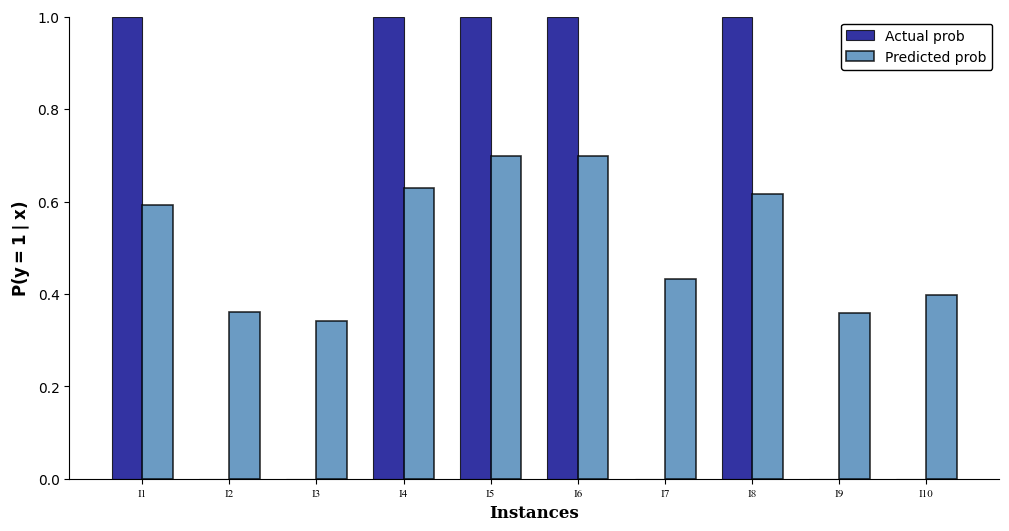
\includegraphics[width=0.80\textwidth]{figures/HeartDisease data/Avgpredicted_probs_polynomial.png}
\caption{Average predicted posterior probabilities for the first 10 instances of the heart dataset using Polynomial logistic scaling}
\label{fig:heart_avg_predicted_probs_polynomial}
\end{figure}

To further extend the analysis of the probabilistic $L_1$-TWSVM with Platt's scaling, Figure \ref{fig:heart_mse_distribution} illustrates the distribution of the Brier Score across $B=50$ bootstrap samples for each hyperparameter configuration within the previously defined optimal set, $\Theta_{\epsilon}$. The figure represents the stability of the model performance, exhibiting limited variability of the BS across bootstrap resamples for each optimal configuration on the \texttt{heart} dataset.

\begin{figure}[H]
\centering

\includegraphics[width = \textwidth]{figures/HeartDisease data/mse_distribution.png}
\caption{Brier Score distribution across $B=50$ bootstrap samples for the optimal hyperparameter combinations on heart dataset}
\label{fig:heart_mse_distribution}
\end{figure}

Table \ref{tab:results} summarizes the results obtained for each dataset, including the optimal hyperparameter configuration and the corresponding mean and variance of the classification accuracy and Brier Score. The probabilistic $L_1$-TWSVM with Platt scaling exhibits a high degree of stability, as evidenced by the consistently low standard deviations observed for both performance metrics across the bootstrap replicates.

\begin{table}[H]
\centering
\caption{Probabilistic $L_1$-TWSVM results}
\label{tab:results}
\begin{tabular}{lccc}
\hline
\textbf{Dataset} & \textbf{$\theta^{*}$} & \textbf{Accuracy (Mean $\pm$ sd)} & \textbf{MSE (Mean $\pm$ sd)} \\
\hline
\texttt{heart} & ($2^{0}, 2^{2}$) & $0.8307 \pm 0.0372$ & $0.1299 \pm 0.0163$ \\
\texttt{wisconsin} & ($2^{0}, 2^{6}$) & $0.9414 \pm 0.0213$ & $0.0308 \pm 0.0118$\\
\texttt{banknote} & ($2^{-6}, 2^{3}$) & $0.9826 \pm 0.0042$ & $0.0098 \pm 0.0019$ \\
\texttt{synthetic} & ($2^{-2}, 2^{-4}$) & $0.9662 \pm 0.0088$ & $0.0336 \pm 0.0055$ \\
\hline
\end{tabular}
\end{table}

As described in Section \ref{chap:experiment}, the bootstrap procedure yields, for each hyperparameter configuration $\theta$ and bootstrap replicate b, independently selected subsets of features for each hyperplane namely, $n_1^{(\theta, b)}, n_2^{(\theta, b)}$. This procedure enables the construction of heatmaps representing the frequency with which each feature is selected by the $L_1$-TWSVM method under each optimal hyperparameter configuration across bootstrap samples. Recall that the hyperparameter configurations are ranked in descending order according to their overall accuracy, $\bar{acc}_{\theta}$. 

\newpage

Figure \ref{fig:fs_heatmap_synthetic} presents the empirical feature selection frequencies for both hyperplanes under the optimal hyperparameter configurations for the \texttt{synthetic} dataset. These frequencies may be interpreted as Monte Carlo estimates of the marginal feature selection probabilities induced by the $L_1$-TWSVM under the bootstrap sampling scheme. By construction, the \texttt{synthetic} dataset contains two informative features, located in the first two feature positions, while the remaining features consist solely of random noise. The heatmaps in Figure \ref{fig:fs_heatmap_synthetic} reveal a clear separation between the estimated selection probabilities of informative and non-informative features.

In particular, for the second hyperplane, the two informative features exhibit consistently high selection probabilities across bootstrap replicates and optimal hyperparameter configurations, whereas the noisy features are selected with substantially lower frequency. This behaviour suggests a stable feature selection mechanism capable of consistently identifying the true signal despite sampling variability. For the first hyperplane, a similar pattern is observed, with noisy features generally exhibiting lower selection frequencies. However, the distinction between informative and non-informative features is less pronounced, indicating greater uncertainty in the feature selection process associated with the first hyperplane.

\begin{figure}[H]
\centering

\begin{subfigure}[t]{0.48\textwidth}
\centering

\includegraphics[width=0.90\textwidth]{figures/Synthetic data/H1_fs_heatmap.png}
\caption{Hyperplane 1 feature selection frequency}
\label{fig:h1_fs_heatmap}
\end{subfigure}
\begin{subfigure}[t]{0.48\textwidth}
\centering

\includegraphics[width=0.90\textwidth]{figures/Synthetic data/H2_fs_heatmap.png}
\caption{Hyperplane 2 feature selection frequency}
\label{fig:h2_fs_heatmap}
\end{subfigure}

\caption{Feature selection frequency heatmaps across bootstrap samples under optimal hyperparameter configurations for the synthetic dataset.}
\label{fig:fs_heatmap_synthetic}
\end{figure}

Analogously, the results obtained for the \texttt{synthetic} dataset are presented to assess the behaviour of the proposed joint post-hoc feature ranking strategy. For each hyperparameter configuration $\theta$ and bootstrap replicate $b$, the bootstrap procedure computes the feature importance measure, defined in Equation \ref{eq:feature_importance} and denoted by $FS_j^{(\theta, b)}$, for the features belonging to the union of the subsets selected by the two hyperplanes, $n_1^{(\theta, b)}$, $n_2^{(\theta, b)}$. Consequently, for a fixed hyperparameter configuration, an overall importance score can be assigned to each feature by averaging its importance values across the $B$ bootstrap samples.

\newpage

The final importance assigned to the $j$-th feature is obtained by aggregating the configuration-specific feature importance scores across all hyperparameter configurations. The contribution of each configuration is weighted by its normalized calibration weight, $w_{\theta}^{BS}$, defined in Equation \ref{eq:normalized_calibration_weight}. The resulting global feature importance score is given by

\begin{align}
FS_j^{final} = \sum_{\theta \in \Theta} w_{\theta}^{BS} \Big(\frac{1}{B}\sum_{b=1}^{B} \frac{|w_{1,j}^{(\theta, b)}| + |w_{2,j}^{(\theta,b)}|}{\sum_{k\in n_1^{(\theta,b)}\cup n_2^{(\theta,b)}} (|w_{1,k}^{(\theta, b)}| + |w_{2,k}^{(\theta,b)}|)} \Big) = \sum_{\theta \in \Theta} w_{\theta}^{BS} \Big(\frac{1}{B}\sum_{b=1}^{B} FS_j^{(\theta, b)}\Big)
\end{align}

where $\sum_{j\in N} FS_j^{final} = 1$ so that $FS_j^{final}$ might be interpreted as a normalized measure of relative importance of the feature $j$-th. The proposed aggregation scheme assigns greater weight to hyperparameter configurations exhibiting superior probabilisitc calibration performance while simultaneously accounting for uncertainty arising from both bootstrap resampling and hyperparameter tuning.

Figure \ref{fig:post_hoc_fs_synthetic} shows that the proposed joint post-hoc ranking strategy successfully recovers the two unique informative features embedded by construction in the \texttt{synthetic} dataset.

\begin{figure}[H]
\centering

\includegraphics[width=0.90\textwidth]{figures/Synthetic data/final_fs.png}
\caption{Joint post-hoc selected features on the \texttt{synthetic} dataset}
\label{fig:post_hoc_fs_synthetic}
\end{figure}

After demonstrating the feature selection capabilities induced by the $L_1$ regularization terms on each proximal hyperplane using the \texttt{synthetic} dataset, Figure \ref{fig:fs_heatmap_heart} illustrates the feature selection frequencies across bootstrap replicates for the optimal hyperparameter configuration identified for the \texttt{heart} dataset. In addition, the joint post-hoc feature ranking strategy was also applied to the \texttt{heart} dataset, with the resulting rankings presented in Figure \ref{fig:post_hoc_fs_heart}. The corresponding feature selection results for the remaining datasets are included in the Appendix.

\begin{figure}[H]
\centering

\begin{subfigure}[t]{0.48\textwidth}
\centering

\includegraphics[width=0.90\textwidth]{figures/HeartDisease data/H1_fs_heatmap.png}
\caption{Hyperplane 1 feature selection frequency}
\label{fig:h1_fs_heatmap}
\end{subfigure}
\begin{subfigure}[t]{0.48\textwidth}
\centering

\includegraphics[width=0.90\textwidth]{figures/HeartDisease data/H2_fs_heatmap.png}
\caption{Hyperplane 2 feature selection frequency}
\label{fig:h2_fs_heatmap}
\end{subfigure}

\caption{Feature selection frequency heatmaps across bootstrap samples under optimal hyperparameter configurations for the heart dataset.}
\label{fig:fs_heatmap_heart}
\end{figure}

\begin{figure}[H]
\centering

\includegraphics[width=0.90\textwidth]{figures/HeartDisease data/final_fs.png}
\caption{Joint post-hoc selected features on the heart dataset}
\label{fig:post_hoc_fs_heart}
\end{figure}

To achieve complete interpretability of the proposed probabilistic twin classifier, a two-dimensional representation of the proximal hyperplanes is constructed using the two informative attributes of the \texttt{synthetic} dataset. Specifically, by restricting the original dataset to the first two features and fitting the corresponding probabilistic $L_1$-TWSVM model, the positive and negative proximal hyperplanes can be expressed in explicit functional form as

\begin{align}
x_2 = -\frac{w_{i,1}}{w_{i,2}} x_1 - \frac{b_i}{w_{i,2}},
\quad \forall \; i \in \{1,2\}.
\end{align}

Figure \ref{fig:ptwsvm_2d_representation_synthetic} depicts the resulting decision boundary and pair of proximal hyperplanes learned by the proposed probabilistic $L_1$-TWSVM in the two-dimensional feature space spanned by the relevant features of the \texttt{synthetic} dataset under the corresponding optimal hyperparameter configuration, $\theta^{*}$.

\begin{figure}[H]
\centering

\includegraphics[width=0.75\textwidth]{figures/Synthetic data/2d_ptwsvm.png}
\caption{Probabilistic $L_1$-TWSVM decision boundary and hyperplanes in the space of the two relevant features of the synthetic dataset}
\label{fig:ptwsvm_2d_representation_synthetic}
\end{figure}

The feature selection results for the \texttt{banknote} dataset, provided in the Appendix, reveal that the numerical features \textit{skewness} and \textit{variance} are the most influential in determining both proximal hyperplanes. Figure \ref{fig:ptwsvm_2d_representation_banknote} depicts the decision boundary and the associated proximal hyperplanes generated by the probabilistic $L_1$-TWSVM model within the two-dimensional feature space spanned by these features.

\begin{figure}[H]
\centering
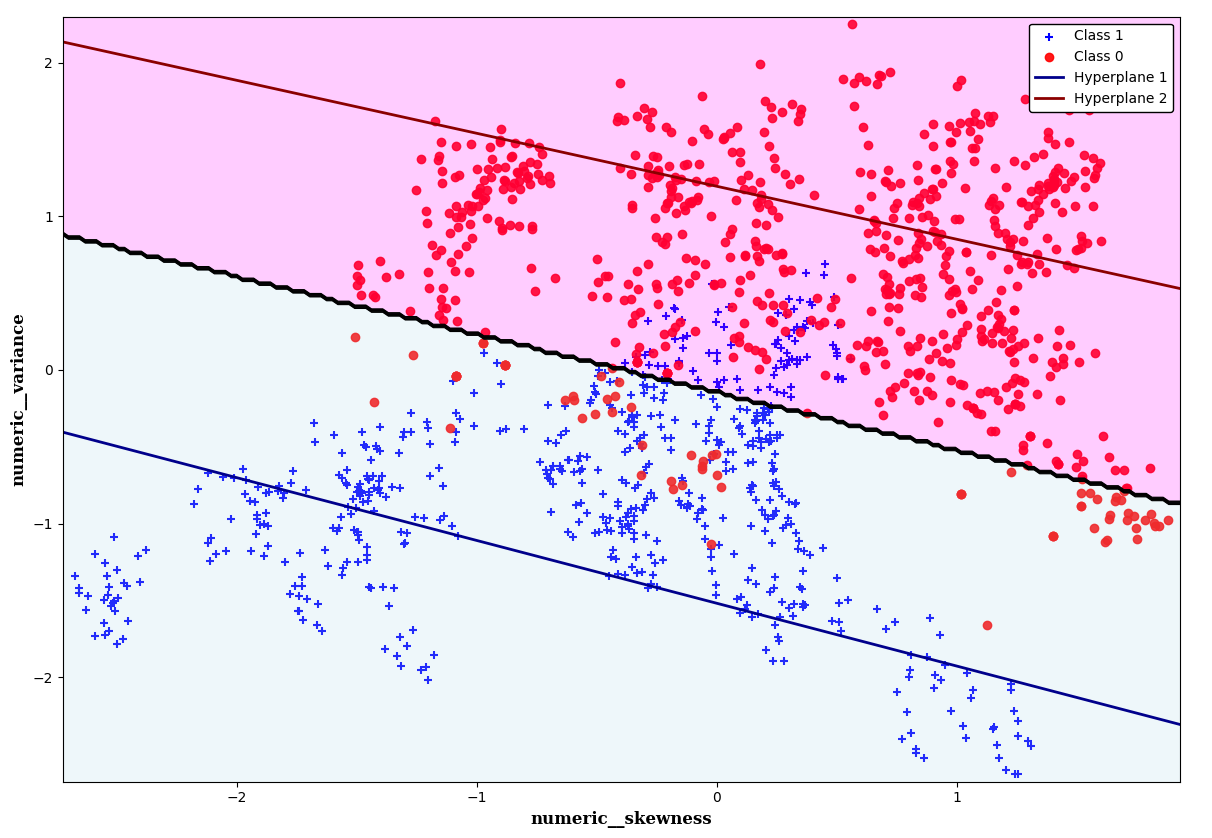
\includegraphics[width=0.75\textwidth]{figures/Banknote data/2d_ptwsvm.png}
\caption{Probabilistic $L_1$-TWSVM decision boundary and hyperplanes in the space of the two relevant features of the banknote dataset}
\label{fig:ptwsvm_2d_representation_banknote}
\end{figure}

\newpage

Table \ref{tab:results-comparison} summarizes the average classification accuracy and MSE, together with their respective standard deviations in parentheses, obtained across the $B$ bootstrap samples for the standard linear SVM, the probabilistic TWSVM (PTWSVM) proposed by \cite{shao2012probabilistic}, and the probabilistic $L_1$-TWSVM implemented in this thesis. The table reports the stability of each model under their optimal hyperparameter configurations for each dataset. As discussed in Section \ref{chap:evaluation}, the leave-one-out bootstrap procedure employed in this study tends to produce optimistic estimates of future predictive performance. Nevertheless, the three proposed SVM-based methods exhibit highly similar performance across the evaluated datasets under their respective optimal configurations, suggesting that their predictive performance is consistent across bootstrap samples.

\begin{table}[H]
\centering
\caption{Performance comparison of Linear SVM, PTWSVM and Probabilistic $L_1$-TWSVM.}
\label{tab:results-comparison}

\small
\setlength{\tabcolsep}{4pt}

\begin{tabular}{l cc cc cc}
\hline
& \multicolumn{2}{c}{\textbf{Linear SVM}}
& \multicolumn{2}{c}{\textbf{PTWSVM}}
& \multicolumn{2}{c}{\textbf{Probabilistic $L_1$-TWSVM}} \\
\cline{2-3}\cline{4-5}\cline{6-7}
\textbf{Dataset}
& \textbf{Accuracy (sd)} & \textbf{MSE (sd)}
& \textbf{Accuracy (sd)} & \textbf{MSE (sd)}
& \textbf{Accuracy (sd)} & \textbf{MSE (sd)} \\
\hline

\texttt{heart}
& \result{0.8253}{0.0287}
& \result{0.1250}{0.0187}
& \result{0.8240}{0.0361}
& \result{0.1322}{0.0171}
& \result{0.8307}{0.0372}
& \result{0.1299}{0.0163}
\\

\texttt{wisconsin}
& \result{0.9670}{0.0115}
& \result{0.0222}{0.0060}
& \result{0.9404}{0.0212}
& \result{0.0355}{0.0088}
& \result{0.9414}{0.0213}
& \result{0.0308}{0.0118}
\\

\texttt{banknote}
& \result{0.9903}{0.0037}
& \result{0.0082}{0.0019}
& \result{0.9796}{0.0050}
& \result{0.0079}{0.0018}
& \result{0.9826}{0.0042}
& \result{0.0098}{0.0019}
\\

\texttt{synthetic}
& \result{0.9717}{0.0088}
& \result{0.0288}{0.0063}
& \result{0.9663}{0.0085}
& \result{0.0334}{0.0058}
& \result{0.9662}{0.0088}
& \result{0.0336}{0.0055}
\\

\hline
\end{tabular}
\end{table}

Finally, Table \ref{tab:hyperparameters-confgs} illustrates the optimal hyperparameter configurations obtained for each SVM-based method implemented in this thesis across all datasets. Recall that the standard linear SVM fixes the coefficient of the margin maximization term to $\frac{1}{2}$, resulting in a single hyperparameter, $C$, which controls the trade-off between margin maximization and margin violation penalization. Similarly, the standard PTWSVM proposed by \cite{shao2012probabilistic} fixes the coefficients accompanying the least-squares fitting terms in both objective functions. In this formulation, the hyperparameters $c_1$ and $c_2$ control the contribution of the linear penalty terms associated with each hyperplane, respectively. As discussed in Section \ref{chap:experiment} and following \cite{bai2014novel}, the hyperparameters controlling the contribution of the $L_1$ fitting terms and the linear penalty terms in the two objective functions of the Probabilistic $L_1$-TWSVM were constrained to be equal across both hyperplanes, namely $c1 = c2$ and $c_3 = c_4$.

\begin{table}[H]
\centering
\caption{Optimal hyperparameters of linear SVM, PTWSVM and Probabilistic $L_1$-TWSVM}
\label{tab:hyperparameters-confgs}
\begin{tabular}{lccc}
\hline
\textbf{Dataset} & $M_1 = C$ & $M_2 = (c_1, c_2)$ & $M_3 = (c_1 = c3, c2 = c4)$ \\
\hline
\texttt{heart} & $2^{-4}$ & $(2^{-1}, 2^{-1})$ & $(2^{0}, 2^{2})$ \\
\texttt{wisconsin} & $2^{-4} $ & $(2^{0}, 2^{-8})$ & $(2^{0}, 2^{6})$ \\
\texttt{banknote} & $2^{2}$ & $(2^{3}, 2^{0})$ & $(2^{-6}, 2^{3})$ \\
\texttt{synthetic} & $2^{4}$ & $(2^{-4}, 2^{-8})$ & $(2^{-2}, 2^{-4})$ \\
\hline
\end{tabular}
\end{table}



\chapter{Conclusions} \label{chap:conclusions}

The probabilistic $L_1$-TWSVM model implemented in this work exhibited substantial stability in the calibration of its predicted probabilities. Both calibration strategies considered in this thesis, namely Platt scaling and polynomial logistic scaling, yielded nearly identical performance across the benchmark datasets. Nevertheless, the probabilistic $L_1$-TWSVM with Platt scaling achieved marginally superior results, exhibiting slightly lower mean and standard deviation values of the Brier Score across bootstrap replicates.

Regarding the bootstrap results for the independent feature selection strategy applied to each hyperplane, the sparsity induced in the weight vectors through the $L_1$-regularization terms introduced in the objective functions, following the approach proposed by \cite{bai2014novel}, successfully identified the features most relevant to each hyperplane. Likewise, the proposed joint post-hoc feature selection ranking strategy identified the relevant features while providing a normalized measure of relative feature importance. The results indicated that, in the \texttt{heart} and \texttt{wisconsin} datasets, nearly all features contribute at a comparable scale to the determination of both hyperplanes. As shown in the Appendix, the feature selection methods identified the features \textit{variance}, \textit{skewness}, and \textit{kurtosis} as the most relevant for determining the hyperplanes in the \texttt{banknote} dataset, while discarding the \textit{entropy} attribute.

Furthermore, as expected, the predictive performance and stability of the proposed model on the benchmark datasets were comparable to those of the standard linear SVM and the standard Probabilistic TWSVM proposed by \cite{shao2012probabilistic}. The Probabilistic $L_1$-TWSVM consistently achieved higher classification accuracy and lower MSE than the standard PTWSVM. However, with the exception of the \texttt{heart} dataset, the standard linear SVM with Platt scaling implemented via the \textit{SVC} class in the scikit-learn library, outperformed the probabilistic model proposed in this thesis. These results are consistent with the findings of \cite{khemchandani2007twin}, which indicate the superior performance of TWSVM on XOR-type problems with cross-axis clustered classes.



%----------
%	Bibliography
%----------	

\clearpage
\addcontentsline{toc}{chapter}{Bibliography}

\printbibliography



%----------
%	Appendix
%----------	

% If your work includes Appendix, you can uncomment the following lines
\chapter* {Appendix}
\pagenumbering{gobble} % Appendix pages are not numbered

In the following, the results corresponding to the stability analysis and feature selection for the remaining benchmark datasets, namely \texttt{wisconsin} and \texttt{banknote} are presented. Figures \ref{fig:wisconsin_mse_distribution} and \ref{fig:wisconsin_avg_predicted_probs_platt} present the stability analysis of the probabilistic model calibration on the \texttt{wisconsin} dataset, whereas Figures \ref{fig:fs_heatmap_wisconsin} and \ref{fig:post_hoc_fs_wisconsin} illustrate the corresponding feature selection results.

\begin{figure}[H]
\centering

\includegraphics[width=0.75\textwidth]{figures/BreastCancer data/mse_distribution.png}
\caption{Brier Score distribution across $B=50$ bootstrap samples for the optimal hyperparameter combinations on wisconsin dataset}
\label{fig:wisconsin_mse_distribution}
\end{figure}

\begin{figure}[H]
\centering

\includegraphics[width=0.80\textwidth]{figures/BreastCancer data/Avgpredicted_probs.png}
\caption{Average predicted posterior probabilities for the first 10 instances of the wisconsin dataset using Polynomial logistic scaling}
\label{fig:wisconsin_avg_predicted_probs_platt}
\end{figure}

\begin{figure}[H]
\centering

\begin{subfigure}[t]{0.48\textwidth}
\centering

\includegraphics[width=0.90\textwidth]{figures/BreastCancer data/H1_fs_heatmap.png}
\caption{Hyperplane 1 feature selection frequency}
\label{fig:h1_fs_heatmap}
\end{subfigure}
\begin{subfigure}[t]{0.48\textwidth}
\centering

\includegraphics[width=0.90\textwidth]{figures/BreastCancer data/H2_fs_heatmap.png}
\caption{Hyperplane 2 feature selection frequency}
\label{fig:h2_fs_heatmap}
\end{subfigure}

\caption{Feature selection frequency heatmaps across bootstrap samples under optimal hyperparameter configurations for the wisconsin dataset.}
\label{fig:fs_heatmap_wisconsin}
\end{figure}

\begin{figure}[H]
\centering

\includegraphics[width=0.90\textwidth]{figures/BreastCancer data/final_fs.png}
\caption{Joint post-hoc selected features on the wisconsin dataset}
\label{fig:post_hoc_fs_wisconsin}
\end{figure}

Similarly, given the feature selection results for the \texttt{wisconsin} dataset, exhibited above, reveal that the numerical features \textit{area3} and \textit{radius3} are the most influential in determining both proximal hyperplanes. Figure \ref{fig:ptwsvm_2d_representation_wisconsin} depicts the decision boundary and the associated proximal hyperplanes generated by the probabilistic $L_1$-TWSVM model within the two-dimensional feature space spanned by these features. This figure provides an intuitive explanation for the superior performance of twin classifiers on XOR-type problems. Since the decision boundary is defined by the set of points equidistant from two non-parallel class-specific hyperplanes, it corresponds to the pair of angle bisectors of those hyperplanes. As shown in Figure \ref{fig:ptwsvm_2d_representation_wisconsin}, this results in a characteristic cross-shaped decision geometry in two-dimensional feature spaces.

\begin{figure}[H]
\centering

\includegraphics[width=0.75\textwidth]{figures/BreastCancer data/2d_ptwsvm.png}
\caption{Probabilistic $L_1$-TWSVM decision boundary and hyperplanes in the space of the two relevant features of the wisconsin dataset}
\label{fig:ptwsvm_2d_representation_wisconsin}
\end{figure}


Figures \ref{fig:banknote_mse_distribution} and \ref{fig:banknote_avg_predicted_probs_platt} present the stability analysis of the probabilistic model calibration on the \texttt{banknote} dataset, whereas Figures \ref{fig:fs_heatmap_banknote} and \ref{fig:post_hoc_fs_banknote} illustrate the corresponding feature selection results.

\begin{figure}[H]
\centering
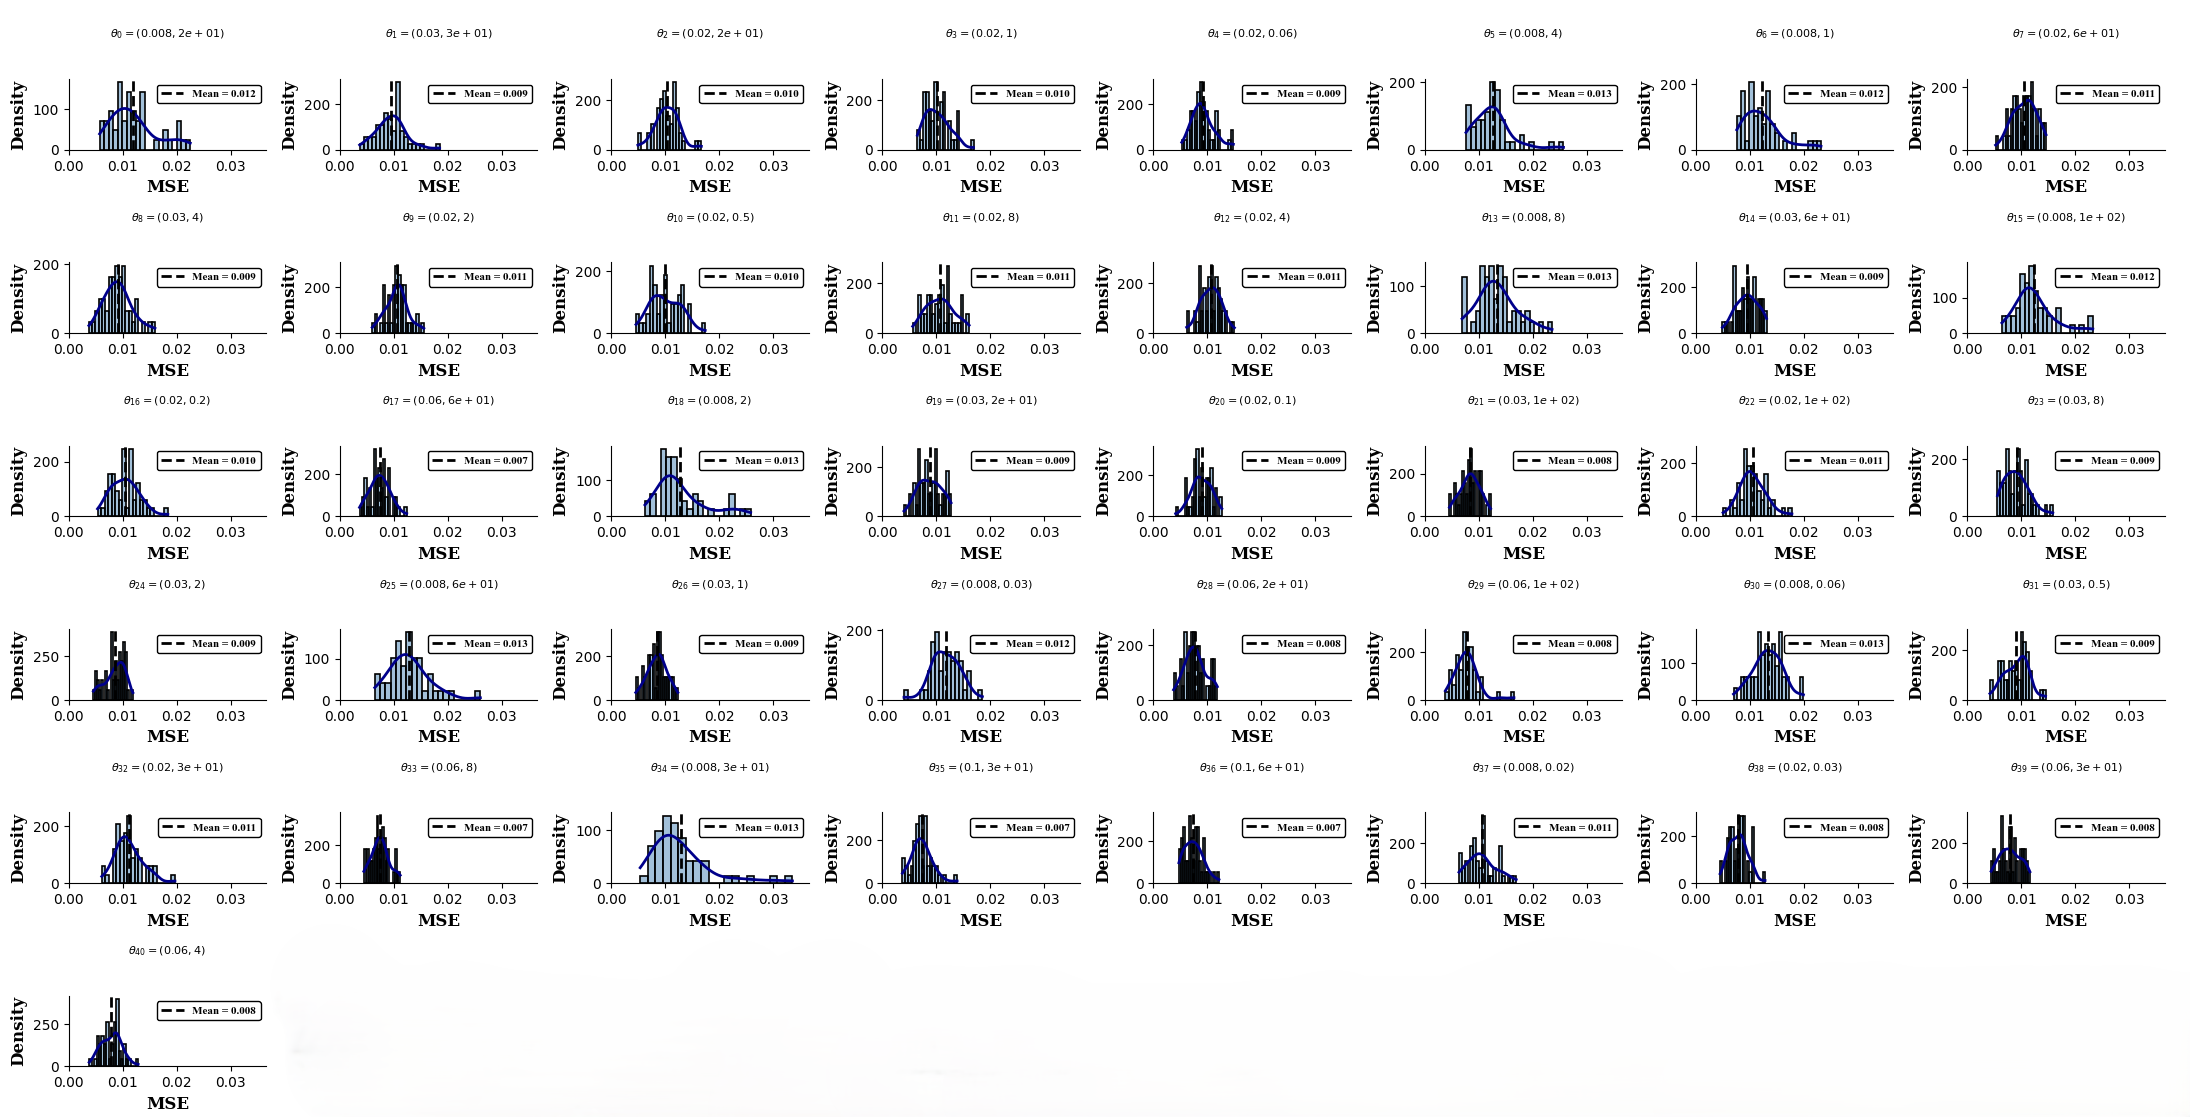
\includegraphics[width=0.75\textwidth]{figures/Banknote data/mse_distribution.png}
\caption{Brier Score distribution across $B=50$ bootstrap samples for the optimal hyperparameter combinations on banknote dataset}
\label{fig:banknote_mse_distribution}
\end{figure}

\begin{figure}[H]
\centering
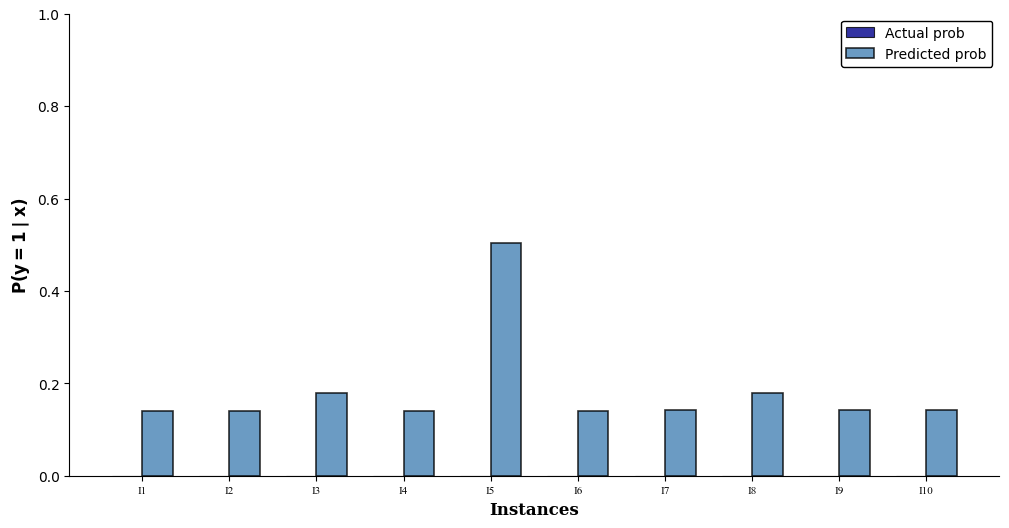
\includegraphics[width=0.80\textwidth]{figures/Banknote data/Avgpredicted_probs_platt.png}
\caption{Average predicted posterior probabilities for the first 10 instances of the banknote dataset using Polynomial logistic scaling}
\label{fig:banknote_avg_predicted_probs_platt}
\end{figure}

\begin{figure}[H]
\centering

\begin{subfigure}[t]{0.48\textwidth}
\centering
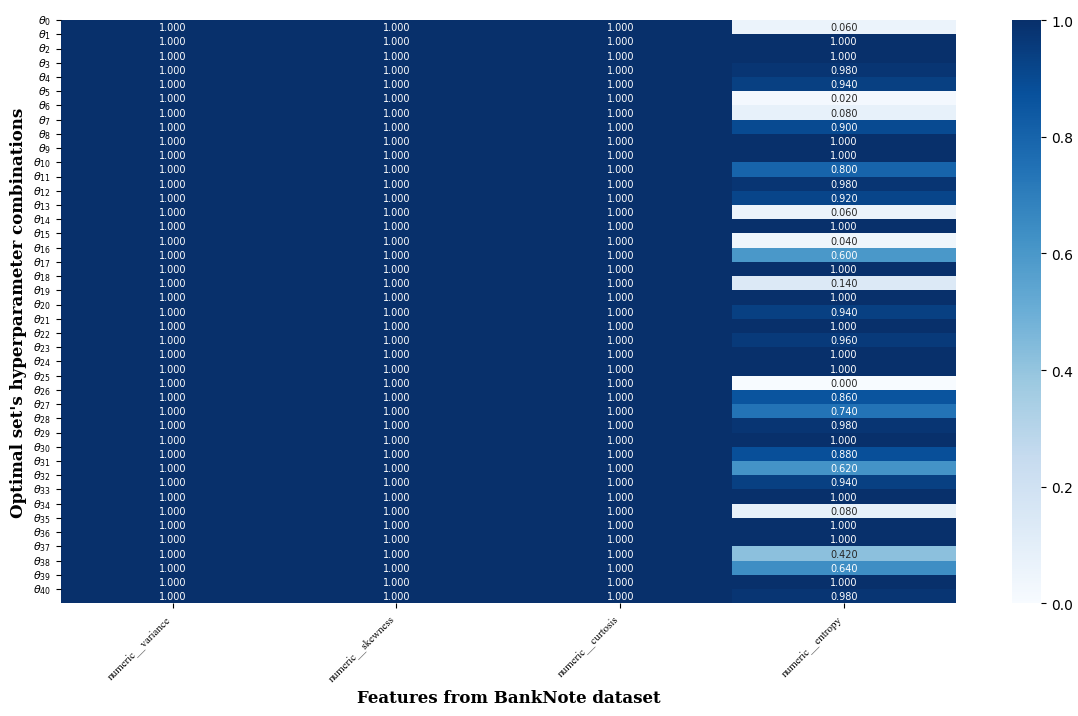
\includegraphics[width=0.90\textwidth]{figures/Banknote data/H1_fs_heatmap.png}
\caption{Hyperplane 1 feature selection frequency}
\label{fig:h1_fs_heatmap}
\end{subfigure}
\begin{subfigure}[t]{0.48\textwidth}
\centering
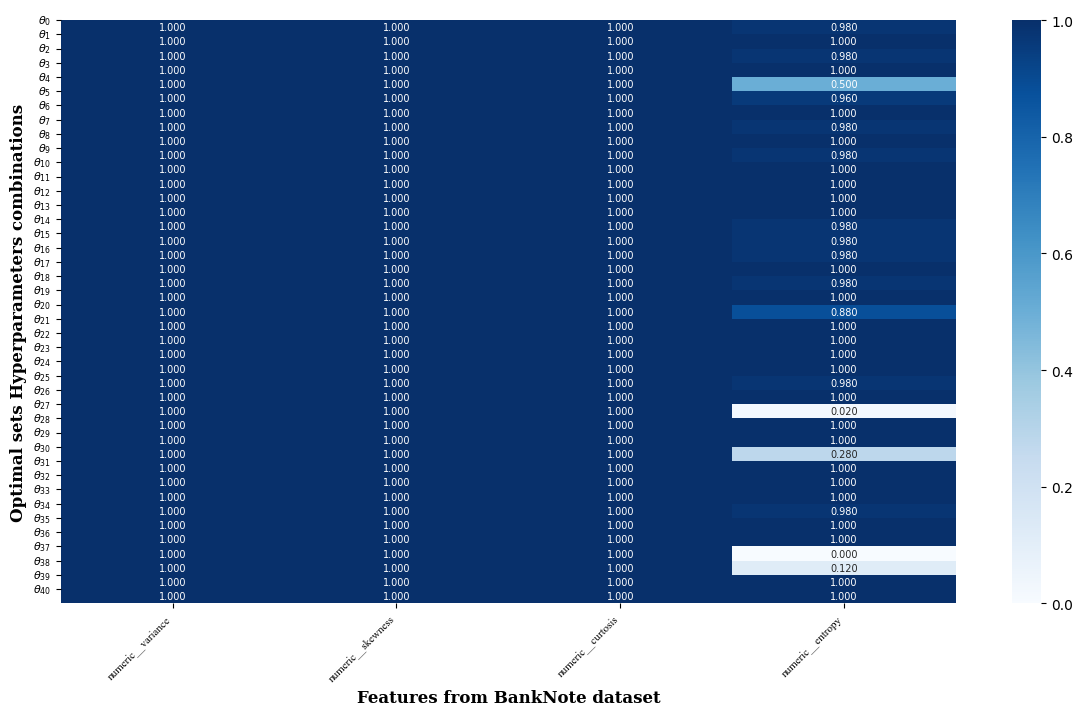
\includegraphics[width=0.90\textwidth]{figures/Banknote data/H2_fs_heatmap.png}
\caption{Hyperplane 2 feature selection frequency}
\label{fig:h2_fs_heatmap}
\end{subfigure}

\caption{Feature selection frequency heatmaps across bootstrap samples under optimal hyperparameter configurations for the banknote dataset.}
\label{fig:fs_heatmap_banknote}
\end{figure}

\begin{figure}[H]
\centering
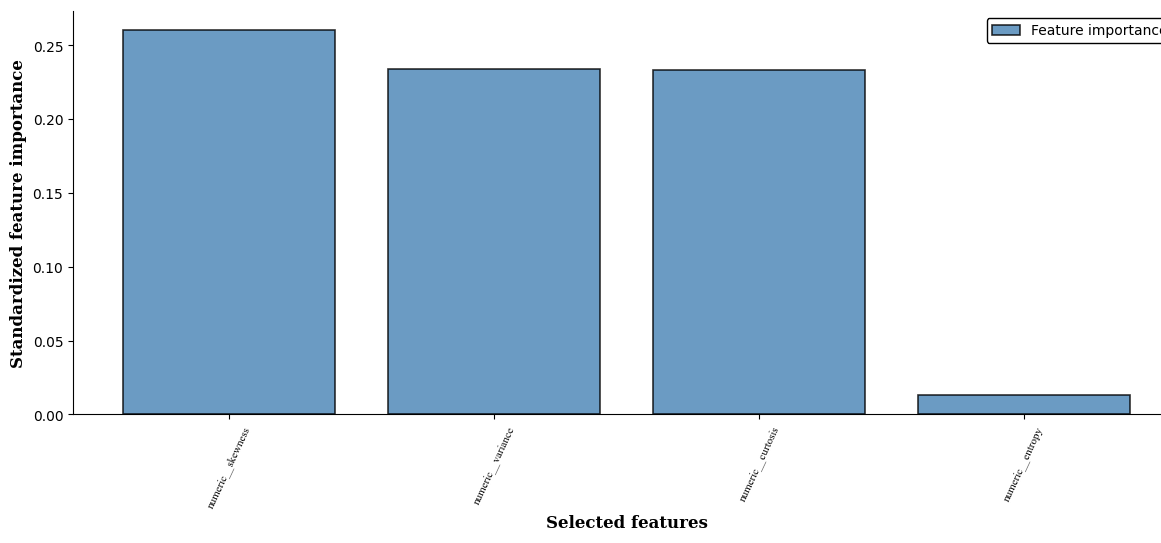
\includegraphics[width=0.90\textwidth]{figures/Banknote data/final_fs.png}
\caption{Joint post-hoc selected features on the banknote dataset}
\label{fig:post_hoc_fs_banknote}
\end{figure}



\end{document}